\documentclass[11pt]{report}

\usepackage{geometry}
\geometry{a4paper}
\usepackage{graphicx}
\graphicspath{ {./images/} }
\DeclareGraphicsExtensions{.png,.pdf,.jpg}
\usepackage{array}
\usepackage{multirow}
\usepackage{mathtools}
\usepackage[T1]{fontenc}
%\usepackage[latin9]{inputenc}
\usepackage{babel}
\usepackage[table]{xcolor}
\usepackage{collcell}
\usepackage{hhline}
\usepackage{pgf}
\usepackage{multicol}
\usepackage{subcaption}
\usepackage{float}
\usepackage{ragged2e}
%\usepackage[spanish]{babel}
\usepackage{hyphenat}
\usepackage{babel}
\usepackage[table]{xcolor}
\hyphenation{compo-nentes investiga-ciones activi-dades a-prender dimensionali-dad propia-mente clasifica-ción preproce-sadas característi-cas prome-dio enferme-dad}

\setlength{\columnsep}{1cm}


\def\colorModel{hsb} %You can use rgb or hsb

\newcommand\ColCell[1]{
  \pgfmathparse{#1<50?1:0}  %Threshold for changing the font color into the cells
    \ifnum\pgfmathresult=0\relax\color{black}\fi
  \pgfmathsetmacro\compA{0}      %Component R or H
  \pgfmathsetmacro\compB{#1/100} %Component G or S
  \pgfmathsetmacro\compC{1}      %Component B or B
  \edef\x{\noexpand\centering\noexpand\cellcolor[\colorModel]{\compA,\compB,\compC}}\x #1
  } 
\newcolumntype{E}{>{\collectcell\ColCell}m{0.4cm}<{\endcollectcell}}  %Cell width
\newcommand*\rot{\rotatebox{90}}

\newcommand{\Maximize}[1]{\underset{#1}{\mathbf{Maximize}}}
\newcommand{\Subjto}{\mathbf{Subject\ to}}

\title{Proyecto de Grado}
\author{Javier Ricardo Becerra Bedoya}

\begin{document}

%\maketitle

\begin{titlepage}
   \begin{center}

       
\includegraphics[width=0.3\textwidth]{university}
       
\vspace{0.5cm}

 	\Huge

       \textbf{Clasificación de Actividad Humana con Acelerómetros de Smartphones}

       \LARGE

       \vspace{1cm}
       Tésis de pregrado presentada para recibir el título de\\
       Ingeniero Electrónico por:


\vspace{0.5cm}

       \textbf{Javier Ricardo Becerra Bedoya}\\
\vspace{1.5cm}
       \textbf{A cargo de:}\\
       \textbf{Catalina Alvarado Rojas Ph.D}  

       \vspace{0.8cm}
 
	\large
       Departamento de Ingeniería Electrónica\\
       Pontificia Universidad Javeriana\\
       Bogotá, Colombia\\
       23 de Noviembre de 2018
 
   \end{center}
\end{titlepage}


\chapter{INTRODUCCIÓN}

\justify
Las enfermedades neurodegenerativas son un término general para una variedad de condiciones que afectan principalmente el sistema nervioso. Las neuronas son los componentes básicos del sistema nervioso central que incluye el cerebro y la medula espinal \cite{Neuro}. Las principales enfermedades neurodegenerativas son: Enfermedad de Alzheimer, Esclerosis lateral amiotrófica, Ataxia de Friedreich, Enfermedad de Huntington, Demencia con cuerpos de Lewy, Atrofia muscular espinal, Enfermedad de Parkinson, entre otras \cite{ParkFound}. En particular, la enfermedad de Parkinson es un trastorno neurodegenerativo que afecta predominantemente las neuronas productoras de dopamina en un área específica del cerebro llamada sustancia negra \cite{ParkFound}. Las personas que padecen esta enfermedad presentan los siguientes síntomas: temblor principalmente en reposo, lentitud de movimientos, rigidez en las extremidades, problemas en el equilibro y en la marcha \cite{ParkFound}.


\justify
\par
\medskip
\noindent
 Más de 10 millones de personas en el mundo viven con la enfermedad de Parkinson \cite{Estadistica}, alrededor de un millón en Estados Unidos \cite{Estadistica}. En Colombia, en ciudades como Bucaramanga, Medellín y Manizales, la prevalencia de la enfermedad de Parkinson es de 0.12\% al 0.47\% y proyectando estos datos a la población actual del país, se estima que podrían ser más de 22.000 casos \cite{colprensa}. La incidencia de la enfermedad de Parkinson aumenta con la edad y se estima que sólo el 4\% de los pacientes se diagnostican antes de los 50 años \cite{Estadistica}. Adicionalmente, alrededor de 60.000 estadounidenses son diagnosticados con Parkinson cada año \cite{Estadistica}. A partir de estos datos, se podría concluir que es importante desarrollar herramientas tecnológicas para la detección temprana de Parkinson, ya que esto podría mejorar la eficiencia de los tratamientos, así como la calidad de vida de los pacientes.


\justify
\par
\medskip
\noindent
El objetivo del reconocimiento de actividad es detectar actividades humanas comunes en entornos de la vida real \cite{kim2010human}. El reconocimiento preciso de actividades es un desafío porque la actividad humana es compleja y altamanete diversa \cite{kim2010human}. La investigación en esta área emplea diferentes algoritmos de aprendizaje automático para reconocer actividades simples y complejas como caminar, correr, cocinar, etc \cite{cao2018gchar}. Particularmente, el reconocimiento de las actividades diarias es esencial para mantener un estilo de vida saludable, rehabilitación de pacientes y cambios de actividad entre los adultos mayores que pueden ayudar para detectar y diagnosticar enfermedades graves \cite{cao2018gchar}.


\justify
\par
\medskip
\noindent
Adicionalmente, los síntomas del Parkinson son poco entendidos. A los pacientes los afectan diversos factores de su vida diaria, como la calidad del sueño y la dieta. Para entender las diferencias, es necesario un monitoreo regular y constante por un tiempo prolongado. Lo que ocurre normalmente es que la gente asiste de una a dos veces al año a un especialista, lo que hace imposible un seguimiento continuo de la enfermedad \cite{elcomercio}. Debido a la baja frecuencia de monitoreo de la enfermedad en la actualidad, es importante el uso de herramientas tecnológicas que permitan hacer el monitoreo de la enfermedad de una manera continua, para extraer mayor información.


\justify
\par
\medskip
\noindent
Por lo tanto, el objetivo de este trabajo de investigación es \textit{"Implementar un sistema de clasificación de actividad humana a partir de señales de acelerómetros para posteriores estudios en pacientes con Parkinson."}

\justify
\par
\medskip
\noindent
El diagrama de bloques que representa el desarrollo del proyecto es el siguiente:
\begin{figure}[h]
  \centering
    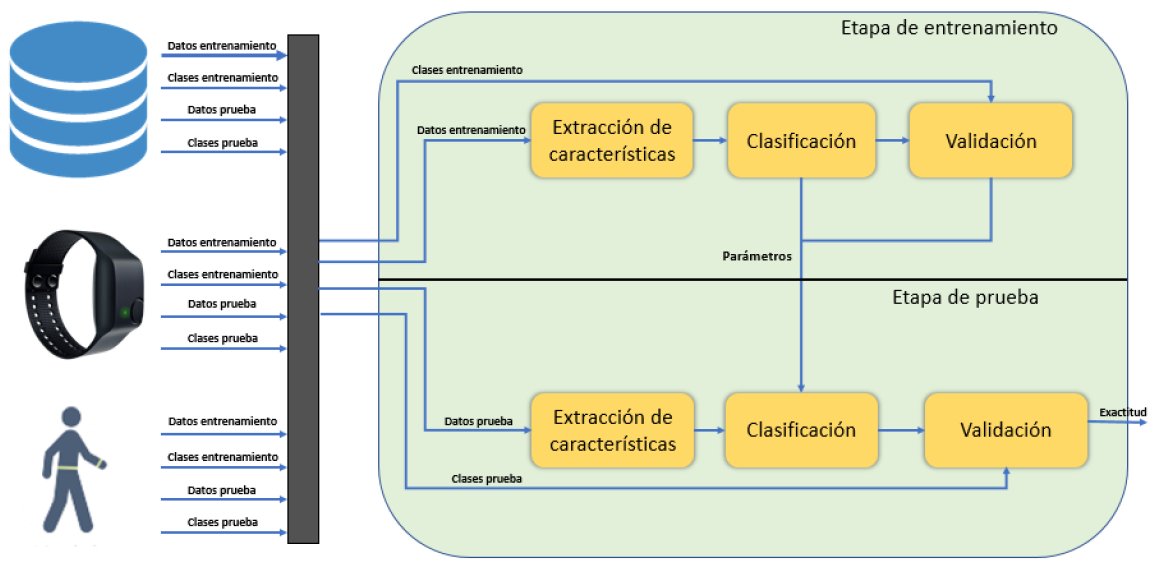
\includegraphics[width=1\textwidth]{diagrama}
   \caption{Diagrama de Bloques del Sistema}
\end{figure}

\chapter{MARCO TEÓRICO}
A lo largo de este capítulo se pretende mostrar los conceptos básicos del análisis de clasificación de actividad humana,
así como las técnicas y tecnologías que han permitido su desarrollo y aplicación durante los últimos años.
\par
\medskip
\noindent
Primero, se dará una introducción y una breve explicación a los antecedentes e investigaciones previas al trabajo a realizar, además se introducirá un concepto de clasificación de actividad humana y del porqué se ha convertido en una herramienta
de importancia en el análisis médico y de ingeniería en la actualidad. Posteriormente, se explicará detalladamente los métodos usados para el reconocimiento de actividad humana.
\section{Antecedentes}
En noviembre 07 del 2012 el Departamento de Medicina Física y de Rehabilitación, de la Universidad Northwestern
en Chicago publicó un artículo llamado “Using mobile phones for activity recognition in Parkinson’s patients” en
el cual expone el trabajo realizado que consistió en identificar 5 actividades (caminando, reposo, sentado, de pie,
o no utilizando el celular) de 18 sujetos sanos y 8 pacientes con enfermedad de Parkinson. Además, se mostraban
las diferencias que hay entre los algoritmos de reconocimiento de actividad corporal entre personas sanas y
pacientes. Los resultados del proyecto arrojaron una exactitud del 96,1 \% de clasificación de actividades en las
personas sanas y un 92,2 \% en los pacientes. 
\par
\medskip
\noindent
En cuanto a los mecanismos de monitoreo de pacientes con Parkinson, se encuentra una aplicación móvil llamada
CloudUPDRS, es un sistema de análisis de datos que pueden usar los pacientes y sus cuidadores para evaluar con
precisión los síntomas motores de Parkinson. Se puede analizar movimientos como temblor, marcha y la capacidad
con la que interactúan con el Smartphone, para evaluar con precisión los síntomas de la enfermedad usando el
método UPDRS (Unified Parkinson’s Disease Rating Scale). Tiene la capacidad de descartar información falsa al
92,5\% \cite{PacientesParkinson}.
\par
\medskip
\noindent
Existe un sistema llamado Mobility Lab de APDM el cual pretende medir la progresión temporal de la
enfermedad de Parkinson. Analizan el equilibrio y la marcha de los pacientes ya que son los dos impedimentos
motores que más afectan la calidad de vida de los enfermos con Parkinson. Utilizan unos sensores llamados Opal,
que se localizan en las piernas, el tronco y los brazos, durante las dos actividades prescritas \cite{MobilityLab}.
\par
\medskip
\noindent
Adicionalmente, en un proyecto realizado por un grupo de universidades latinoamericanas y liderado por Mónica
Huerta, con el título “Monitoreo remoto de pacientes con la enfermedad de Parkinson”, se pretendía mejorar el
diagnóstico y monitoreo de la enfermedad \cite{MonitoreoRemoto}. Usaron en la investigación un sensor de Kinect, smartphones,
hardware libre y smartwatch.
\par
\medskip
\noindent
Finalmente, motivados por la necesidad de detectar automáticamente las diferentes actividades humanas, la
plataforma Kaggle lanzó en el 2016 un concurso abierto \cite{Kaggle}. Para esto, pusieron a disposición una base de datos
de señales de acelerómetros, correspondientes a 6 actividades de 30 personas. Grupos de diferentes partes del
mundo, desarrollaron métodos de clasificación de actividad humana, obteniendo 98\% de exactitud entre los
resultados más destacados.
\section{Algoritmos de Inteligencia artificial en HAR}
En las últimas décadas, un cambio drástico cambió la manera en la que almacenamos, percibimos y procesamos los datos. Una cantidad gigante de datos es generada cada segundo y si se analiza eficientemente estos datos pueden revelar información relevante. Una parte importante en la predicción es seleccionar modelos adecuados \cite{ApplicationHAR}. En la siguiente figura se puede observar un diagrama general en la implementación de machine learning.
\begin{figure}[H]
  \centering
    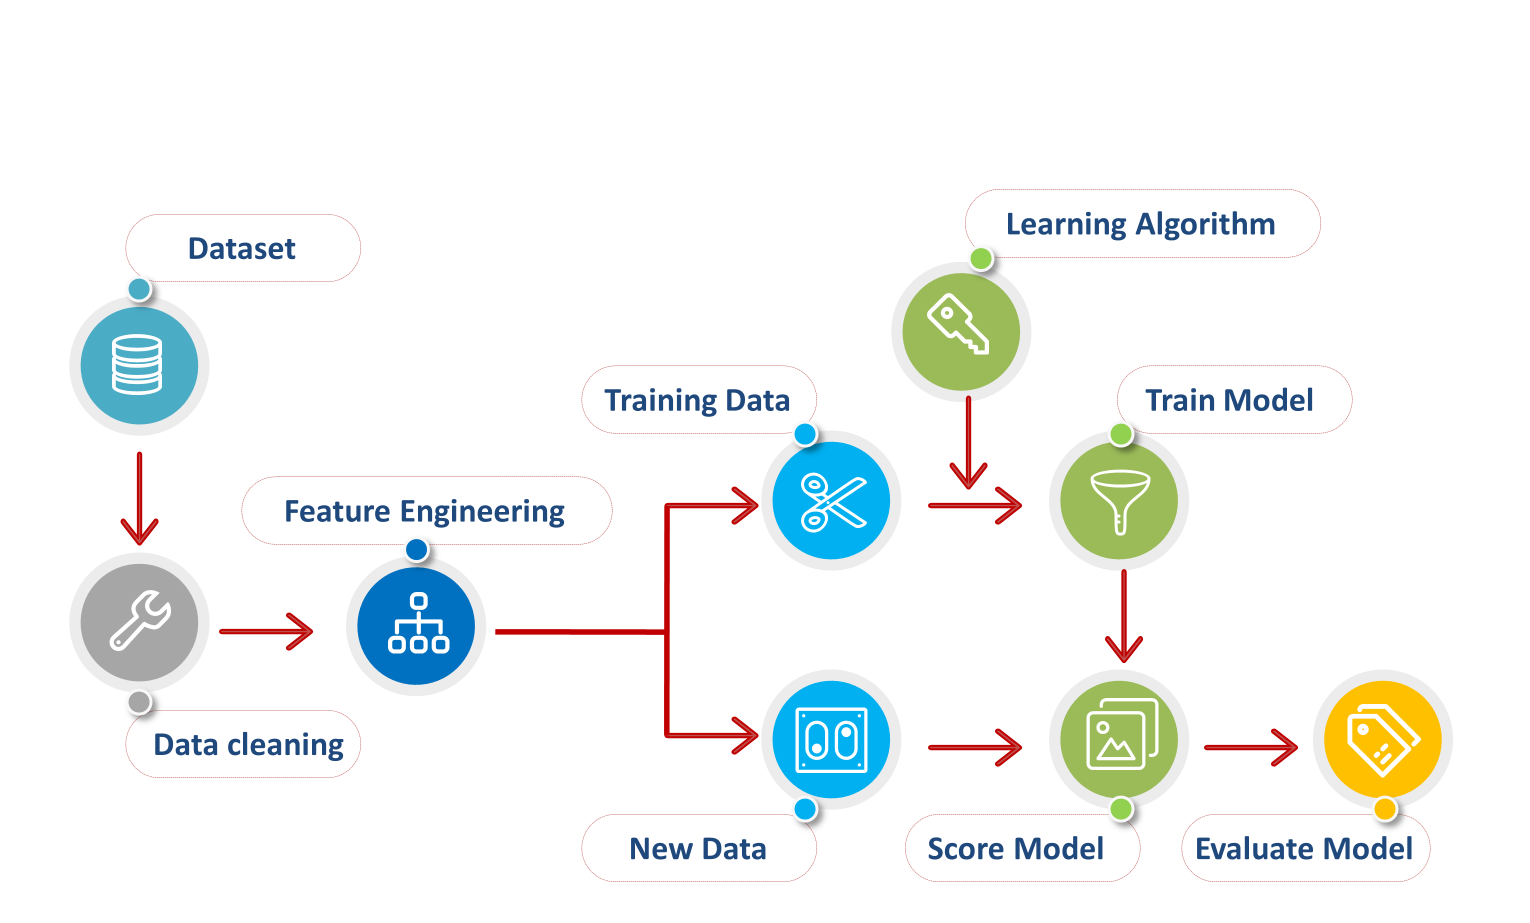
\includegraphics[width=1\textwidth]{machinelearning}
   \caption{Diagrama de Bloques de un sistema de Machine Learning \cite{wowslides_2017}}
\end{figure}

El objetivo de Machine Learning es programar computadoras para que puedan "aprender" a partir de ciertas entradas disponibles. En términos generales el aprendizaje es el proceso de convertir las entradas en experiencia o conocimiento. La entrada a un algoritmo de aprendizaje son datos de entrenamiento, que representan experiencia, y el resultado es algo de experiencia, que generalmente toma la forma de otro programa de computadora que puede realizar alguna tarea \cite{shalev2014understanding}. Para entender un poco más el procedimiento de clasificación se ilustra en la figura un diagrama de bloques en el cual, el dataset son los datos que se usan para entrenar al sistema (en el caso particular de la aplicación, son los datos provenientes de los sensores de acelerómetro y giroscopio). El Data cleaning es el proceso en el cual se filtran (limpian) las señales de entrada para eliminar los datos que no sirven para hacer la predicción para que el modelo no reciba información que no le es útil. Feature Engineering, se trata del proceso previo a la creación del modelo de predicción en el que se hace un análisis y estructuración de las características de los datos. Una vez se tiene una base de datos preprocesada se divide el proceso en dos, una fase de entrenamiento, en la que el modelo es entrenado con diversos algoritmos, iterando para escoger el mejor y el modelo es utilizado para obtener clasificaciones con datos nuevos (fase de testing).

\par
\medskip
\noindent
Como se puede observar en la figura, la extracción de características (Feature Engineering) es una parte del proceso de clasificación a la hora de procesar las señales adquiridas. La selección de las características más relevantes a la hora de analizar y clasificar señales de actividad humana han sido objeto de estudio durante varios años y se presentan en la siguiente tabla.

\begin{table}[H]
\begin{center}
\begin{tabular}{ |c|c|c|c| } 
\hline
Categoría & Característica & Abreviación & Ecuación \\
\hline
\multirow{10}{4em}{Tiempo} & Mean & M & $M = \frac{\sum x}{N}$\\ 
& Variance & V & $V = \frac{\sum (x-\bar{x})^2}{N-1}$\\ 
&  Mean absolute deviation &  MAD& $MAD = \frac{\sum |x-\bar{x}|}{T}$ \\ 
&  Root mean square &  RMS& $RMS = \sqrt\frac{\int_{0}^{T} x^2}{T}$\\
&  Zero Crossing Rate &  ZCR& $ZCR = \frac{1}{T-1}\sum_{t=1}^{T-1} I\{a_i(t)a_i(t+1)<0\}$\\
&  Interquartile Range  &  IQR& $IQR = Q_3-Q_1$\\
&  75'th percentile  &  PE & $PE = \frac{3(n+1)}{4}$\\
&  Kurtosis  &  KS & $KS_i = \frac{\frac{1}{T}\sum_{t=1}^{T}(a_i(t)-M_i)^4}{(\frac{1}{T}\sum_{t=1}^{T}(a_i(t)-M_i)^2)^2}$\\
&  Signal magnitude area  &  SMA & $SMA = \frac{1}{T}\sum_{t=1}^{T}|a_x(t)|+|a_y(t)|+|a_z(t)|$\\
&  Min-max  &  MM &\\
\hline
\multirow{4}{4em}{Frecuencia} & Spectral energy & SE & $SE_i = \sum_{f=1}^{F}|A_i(f)|^2$\\ 
& Spectral entropy & E & $E_i =- \sum_{f=1}^{F}\frac{|A_i(f)|^2}{\sum_{j=1}^{F}|A_i(j)|^2}log2(\frac{|A_i(f)|^2}{\sum_{j=1}^{F}|A_i(j)|^2})$\\ 
& Spectral centroid & SC & $SC_i = \frac{\sum_{f=1}^{F}f|A_i(f)|}{\sum_{f=1}^{F}|A_i(f)|}$\\
& Principal frequency & PF & $PF_i = max_f|A_i(f)|,	f\neq0$\\ 
\hline
\multirow{3}{4em}{Otra} & Correlation between axis & CORR & $CORR_{i,j}=\frac{\sum_{t=1}^{T}(a_i(t)-M_i)(a_j(t)-M_j)}{\sqrt{\sum_{t=1}^{T}(a_i(t)-M_i)^2(a_j(t)-M_j)^2}}$\\ 
& Autoregressive coefficients & AR1, AR2 & $AR(p)\rightarrow a_i(t)= \sum_{k=1}^{p}\phi_ka_i(t-k)+\epsilon(t)$\\ 
& Tilt Angle & TA & $TA=arccos(\frac{a_z(t)}{\sqrt{a_x(t)^2+a_y(t)^2+a_z(t)^2}})$\\ 
\hline
\end{tabular}
\caption{Características relevantes en la clasificación de actividad humana \cite{feature}}
\end{center}
\end{table}

En algunas aplicaciones, reducir la dimensionalidad de los datos mediante la selección de un subconjunto de las variables originales puede ser ventajoso por razones que incluyen el costo de realizar, almacenar y procesar mediciones. El arte de machine learning comienza con el diseño de representaciones de datos apropiadas. A menudo se logra un mejor rendimiento utilizando características derivadas de la entrada original \cite{pca}.

\par
\medskip
\noindent
La idea central del análisis de componentes principales (PCA) es reducir la dimensionalidad de un conjunto de datos que consiste en un gran número de variables interrelacionadas, al tiempo que se conserva la mayor cantidad posible de la variación presente en el conjunto de datos. Esto se logra aplicando una transformación lineal a los datos, para representarlos en un nuevo espacio de variables, los componentes principales (PC), que no están correlacionados, y que están ordenados para que los primeros conserven la mayor parte de la variación presente en todas las variables originales \cite{pca2}.


\subsection {Árbol de decisiones}
\begin{figure}[H]
  \centering
    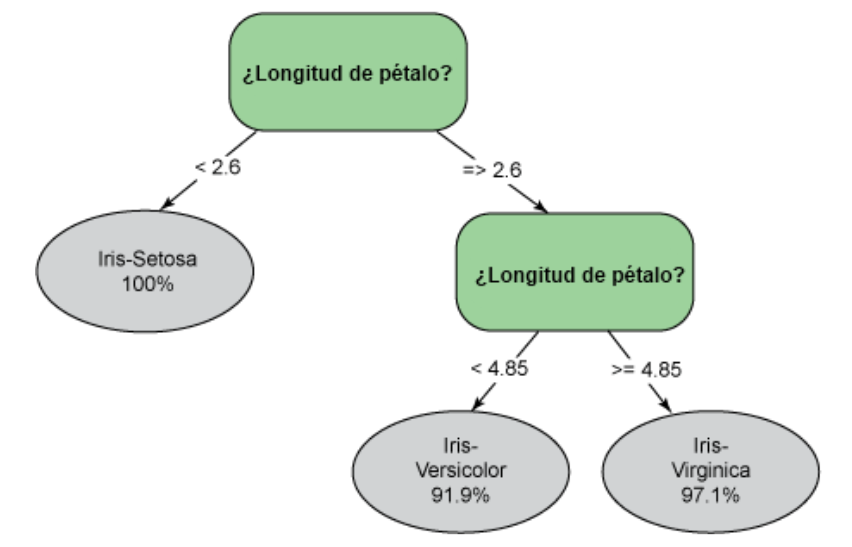
\includegraphics[width=0.8\textwidth]{fig06}
   \caption{Ejemplo Árbol de Decisiones \cite{}}
\end{figure}
 Un árbol de decisión es un modelo de clasificación. Dado un conjunto de datos se fabrican diagramas de construcciones lógicas, que sirven para representar y categorizar una serie de condiciones que ocurren de forma sucesiva, para la resolución de un problema. Los árboles de decisión están formados por nodos, vectores de números, flechas y etiquetas. Cada nodo se puede definir como la característica sobre la que se ha de tomar una decisión de entre varias posibles, lo que va haciendo que a medida que aumenta el número de nodos aumente el número de posibles finales a los que puede llegar el individuo. Los vectores de números serían la solución final a la que se llega en función de las diversas posibilidades que se tienen, dan las utilidades en esa solución. Las flechas son las uniones entre un nodo y otro y representan cada acción distinta. Las etiquetas se encuentran en cada nodo y cada flecha y dan nombre a cada acción \cite{ApplicationHAR}.
\subsection {K-nearest neighbor}
Este clasificador es uno de los métodos de clasificación más fundamentales y se aplica en clasificaciones cuando hay poco o ningún conocimiento previo sobre la distribución de datos. El clasificador KNN se basa comúnmente en la distancia euclidiana entre una muestra de prueba y las muestras de entrenamiento especificadas \cite{ApplicationHAR}. Siendo $x_i$ una muestra de entrada con $p$ características ($x_{i1}, x_{i2}, ..., x_{ip}$), $n$ el total número de muestras de entrada ($i = 1, 2, ..., n$) y $p$ el número total de características ($j = 1, 2, ..., p$). La distancia euclidiana entre la muestra $x_i$ y $x_l$ ($l = 1, 2, ..., n$) está definida como:

\begin{equation}
d(x_i,x_l) = \sqrt{(x_{i1}-x_{l1})^2 + (x_{i2}-x_{l2})^2 + ... + (x_{ip}-x_{lp})^2}
\end{equation}

Una descripción gráfica del clasificador KNN es ilustrado en la Diagrama de Voronoi

\begin{figure}[H]
  \centering
    \includegraphics[width=0.5\textwidth]{knn_voronoi}
   \caption{Diagrama de Voronoi \cite{randomf}}
\end{figure}  

En el diagrama se observan 19 muestras marcadas con un "+", y una celda de Voronoi, $R$, rodeando cada muestra. Una celda de Voronoi encapsula todos los puntos vecinos que son los más cercanos a cada muestra y es definida como:

\begin{equation}
R_i = \{ x \in  R^p : d(x,x_m), \forall i \neq m \}
\end{equation}

Donde $R_i$ es la celda de Voronoi para la muestra $x_i$, y $x$ representa todos los puntos posibles dentro de la celda $R_i$.

\subsection {Support Vector Machine}
\begin{figure}[H]
  \centering
    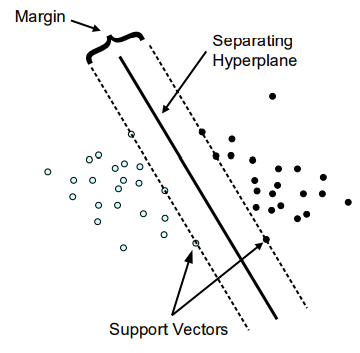
\includegraphics[width=0.5\textwidth]{support}
   \caption{Ejemplo Random Forest \cite{supportv}}
\end{figure}

Son un conjunto de algoritmos de aprendizaje supervisado. Estos métodos están propiamente relacionados con problemas de clasificación y regresión. Básicamente, SVM busca el hiperplano de separación óptimo entre las dos clases al maximizar el margen entre los puntos más cercanos de las clases (ver figura), los puntos que se encuentran en los límites se denominan vectores de soporte, y la mitad del margen es el óptimo separando el hiperplano.

Para maximizar el margen, debemos minimizar el $\parallel w \parallel$

\begin{equation}\label{formula:QPQC}
\begin{aligned}
&\Maximize{w \in H, b \in \Re} && min \{ \parallel x - x_i \parallel |x \in H, \langle w,x \rangle + b = 0, i = 1, ..., m \}
\end{aligned}
\end{equation}

En Machine Learning, los métodos de Kernel son una clase de algoritmos para el análisis de patrones. La tarea general del análisis de patrones es encontrar y estudiar tipos generales de relaciones (por ejemplo, agrupaciones, clasificaciones, correlaciones) en conjuntos de datos. En su forma más simple, el método de Kernel significa transoformar los datos en otra dimensión que tiene un claro margen de división entre las clases de datos \cite{kernel}.

\chapter{OBJETIVOS}

\section{Objetivo general}
Implementar un sistema de clasificación de actividad humana a partir de señales de acelerómetros para posteriores estudios en pacientes con Parkinson.

\section{Objetivos Específicos}
\begin{itemize}
\item Desarrollar algoritmos de clasificación de 6 actividades humanas a partir de señales de movimiento.
\item Diseñar un protocolo experimental con sujetos sanos usando un sensor inercial digital.
\item Validar la clasificación de movimientos de actividad humana, comparando los métodos de clasificación, los tipos de sensores y la posición del sensor, por medio de medidas estadísticas.
\item Comparar el sistema de clasificación respecto al desempeño de sistemas de clasificación ya existentes en la plataforma Kaggle.
\end{itemize}


\chapter{DESARROLLO}
En este capítulo se pretende mostrar el desarrollo de la metodología propuesta para llevar a cabo el cumplimiento de cada uno de los objetivos mencionados anteriormente. En primer lugar se describirá la base de datos (disponible en la plataforma de Kaggle) utilizada para la clasificación de las actividades humanas. Posteriormente, se describirá el procesamiento de las señales de acelerómetro y giroscopio del protocolo de pruebas implementadas, además de un análisis del espacio de carcterísticas.


\section{Base de Datos}
\par
\medskip
\noindent
La base de datos usada fue provista por un concurso realizado por la plataforma Kaggle \cite{Kaggle}. Los experimentos se llevaron a cabo con un grupo de 30 voluntarios dentro de un grupo de edad de 19-48 años. Cada persona realizó las seis actividades mencionadas en la tabla 4.1 con un teléfono inteligente conectado a la cintura, cada sujeto realizó el protocolo dos veces \cite{Angarita}. Además hubo un lapso de 5 segundos entre cada actividad para facilitar el etiquetado del proceso \cite{Anguita}. La base de datos obtenida se dividió en dos conjuntos, donde el 70\% de los datos de usaron para entrenamiento y el 30\% como datos de prueba \cite{Angarita}. El celular usado fue el Samsung Galaxy S2 haciendo uso del acelerómetro y giroscopio para medir la aceleración lineal y angular, respectivamente, a una frecuencia de muestreo de 50 Hz, lo que es suficiente para capturar el movimiento del cuerpo humano \cite{Angarita}.

Las especificaciones del sensor acelerómetro incorporado por el Samsung Galaxy SII, son las siguientes:

\begin{itemize}
\item Ultra bajo consumo, 2 uA (standby) y 40 uA midiendo.
\item Escala plena seleccionable, 2g/4g/8g/16g.
\item 16 bits de salida.
\item Rango de temperatura de -40 - 85 $^\circ$C.
\item Frecuencia de muestreo 50 Hz.
\end{itemize}

%Y las especificaciones del sensor de giroscopio son las siguientes:

%\begin{itemize}
%\item Ultra bajo consumo, 2 uA (standby) y 40 uA midiendo.
%\item Escala plena seleccionable, 2g/4g/8g/16g.
%\item 16 bits de salida.
%\item Rango de temperatura de -40 - 85 $^\circ$C.
%\item Frecuencia de muestreo 50 Hz.
%\end{itemize}


\begin{table}[h!]
\begin{center}
\begin{tabular}{ |c|c|c|c|c|c| } 
\hline
\textbf{No.} & \textbf{Estáticas} & \textbf{Tiempo (S)} & \textbf{No.} & \textbf{Dinámicas} & \textbf{Tiempo (S)} \\
\hline
0 & Comienzo (de pie) & 0 & 7 & Caminar (1) & 15 \\ 
1&  Reposo & 15 & 8 & Caminar(2) & 15\\ 
2&  Sentar & 15 & 9 & Bajar Escaleras (1) & 12\\ 
3&  Reposo & 15 & 10 & Subir Escaleras (2) & 12\\ 
4&  Acostarse & 15 & 11 & Bajar Escaleras (1) & 12\\ 
5&  Sentar & 15 & 12 & Subir Escaleras(2) & 12\\ 
6&  Acostarse & 15 & 13 & Bajar Escaleras (3) & 12\\ 
&   &  & 14 & Subir escaleras (3) & 12\\
&   &  & 15 & Parar & 0\\ 
\hline
\hline
&   &  &  & \textbf{Total} & \textbf{192}\\ 
\hline
\end{tabular}
\caption{Protocolo de actividades realizadas \cite{Anguita}}
\end{center}
\end{table}

\par
\medskip
\noindent
El proceso de reconocimiento comienza con la adquisición de señales del sensor, que posteriormente se procesan aplicando filtros para separar la señal de interés y el ruido y luego se dividen en ventanas con un ancho de 2.56 segundos y una superposición del 50\% \cite{Angarita}. Desde cada ventana, se obtiene un vector de 17 características calculando variables de las señales del acelerómetro en el dominio del tiempo y la frecuencia \cite{Angarita}. La transformada rápida de Fourier se usa para encontrar los componentes en frecuencia de la señal. Finalmente, estos patrones se utilizan como entrada del clasificador para el reconocimiento de las actividades.


\section{Base de Datos Protocolo Implementado}

Las señales de los sensores fueron preprocesadas con la aplicación de una serie de filtros para acondicionamiento. Primero, el ruído fue reducido con un filtro mediano y un filtro Butterworth con una frecuencia de corte de 20 Hz. Esta frecuencia fue escogida porque el ancho de banda de las señales de movimiento humano generalmente se mantiene en el rango entre 0 Hz hasta 15 Hz. Después de este procesamiento, se obtiene un vector triaxial de aceleración A. Esta señal puede ser expresada como la suma de dos vectores de aceleración, la componente gravitacional G y la componente de la aceleración del cuerpo BA, esta separación fue realizada usando otro filtro pasabajos asumiendo que la componente gravitacional solo influye en las más bajas frecuencias, para esto se usó un filtro con frecuencia de corte 0.3 Hz \cite{Anguita}.


\par
\medskip
\noindent
Después de la segmentación, se generaron ventanas con las señales de aceleración preprocesadas, cada una con un ancho de 2.56 segundos y sobrelapadas un 50\%. La longitud de las ventanas fue seleccionada por las siguientes razones:
 
\begin{itemize}
\item El rango de una persona promedio caminando es de [90,130] pasos/min lo cual denota un mínimo de velocidad de 1.5 pasos/segundo.
\item Se desea al menos un ciclo de caminado de dos pasos en cada ventana.
\item Las señales en el dominio de frecuencia requieren Transformada de Fourier rápida (FFT) que está optimizada para la potencia de dos vectores (2.56s * 50 Hz = 128 ciclos).
\item Las personas con un ritmo más lento, como los discapacitados y los ancianos son tenidos en cuenta en este enfoque, por lo que se  eligió una velocidad mínima de cadencia del cuerpo humano del 50\%.
\end{itemize}

\par
\medskip
\noindent
De cada ventana, un vector de características fue extraído, el cual contiene 40 características estimadas de las medidas en el dominio del tiempo y de la frecuencia. Las transformada rápida de Fourier fue usada para encontrar los componentes de frecuencia para cada ventana \cite{Anguita}. 

\section{Espacio de características}

Como motivación en el objetivo de clasificar cada una de las señales, se hicieron 3 gráficas del espacio de características, cada una obteniendo información de una aceleración (promedio de aceleración lineal del cuerpo, promedio de aceleración angular, promedio de aceleración lineal de la gravedad) en cada uno de los ejes correspondientes y los resultados se observan en las figuras  4.1, 4.2 y 4.3.

\begin{figure}[H]
  \centering
    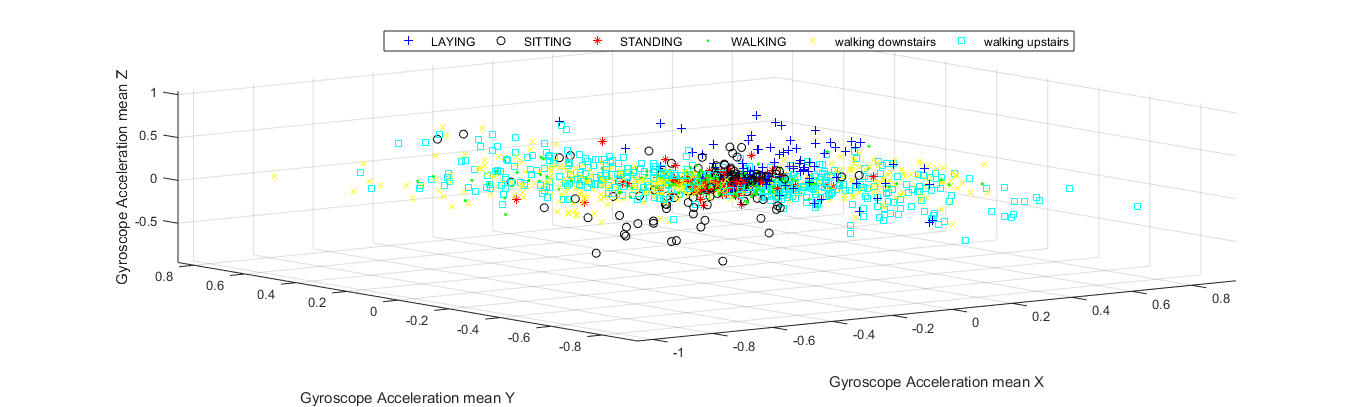
\includegraphics[width=1.2\textwidth]{aceleracion_angular}
   \caption{Espacio de características Aceleración Angular}
\end{figure}

\begin{figure}[H]
  \centering
    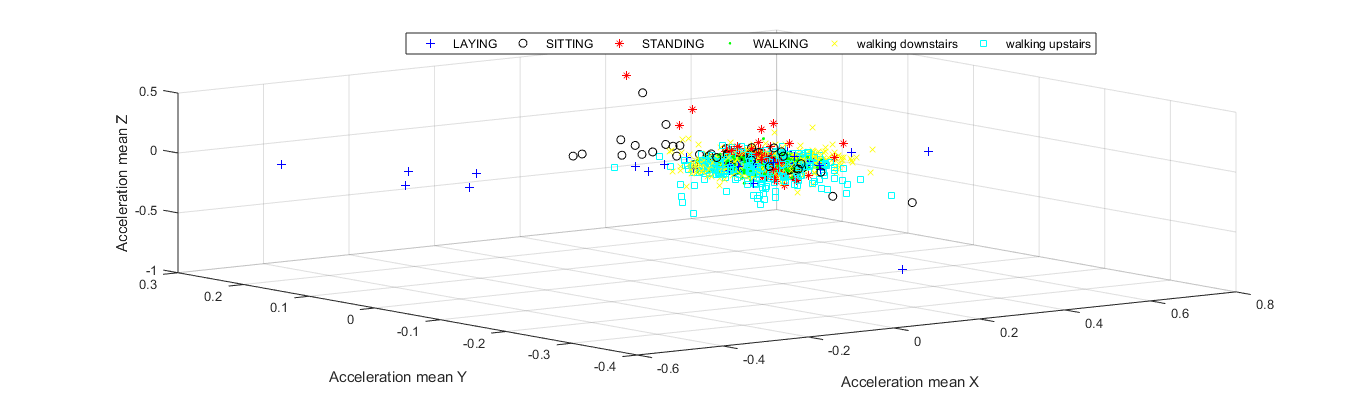
\includegraphics[width=1.2\textwidth]{aceleracion_lineal}
   \caption{Espacio de características Aceleración Lineal}
\end{figure}

\begin{figure}[H]
  \centering
    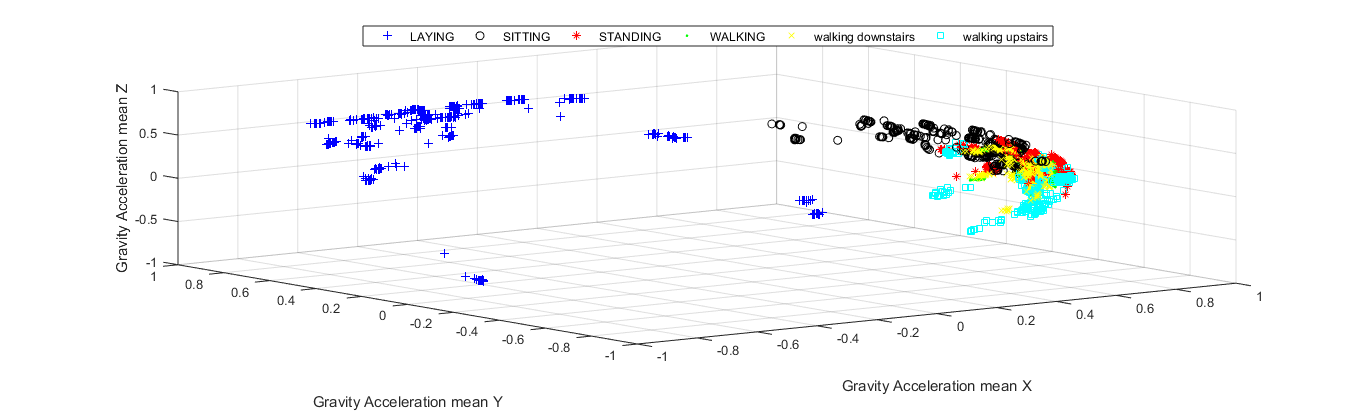
\includegraphics[width=1.2\textwidth]{aceleracion_gravedad}
   \caption{Espacio de características Aceleración Gravedad}
\end{figure}

\section{Classification Learner}

El procedimiento para el entrenamiento del modelo para cada algoritmo con su respectivo Kernel, fue realizado con la App de Matlab Classification Learner, usando esta aplicación se pueden entrenar aprendizajes de máquina supervisado usando varios clasificadores. La aplicación permite explorar los datos, seleccionar las características, entrenar modelos y validar resultados. Adicionalmente, los resultados de los clasificadores son mostrados por medio de matrices de confusión, que permiten la visualización del desempeño de un algoritmo en aprendizaje supervisado. Cada columna de la matriz representa el número de predicciones de cada clase, mientras que cada fila representa a las instancias en la clase real, una ventaja importante a la hora de observar los resultados por medio de matrices de confusión es que facilitan ver si el sistema está confundiendo dos clases. Los clasificadores que serán utilizados para entrenar los modelos se presentan en la siguiente tabla:

\begin{table}[H]
\begin{center}
  \begin{tabular}{|l|l|l|l|l|l|l|}
    \hline
 \textbf{Clasificador} & \textbf{Kernel} & \textbf{Abreviación}\\
    \hline
    Support Vector Machine & Linear & Linear SVM \\
    \hline
    Support Vector Machine & Quadratic & Quadratic SVM \\
    \hline
    Support Vector Machine & Cubic & Cubic SVM \\
    \hline
     Support Vector Machine & Medium Gaussian & M.G. SVM \\
    \hline
    Árbol de Decisiones & Fine & Fine DT \\
    \hline
    Árbol de Decisiones & Medium & Medium DT \\
    \hline
    Árbol de decisiones & Complex & Complex DT \\
    \hline
     K-nearest Neighbor & Fine & Fine KNN \\
    \hline
    K-nearest Neighbor & Cosine & Cosine KNN \\
    \hline
    K-nearest Neighbor & Weighted & Weighted KNN \\
    \hline
  \end{tabular}
\label{Efectos de PCA}
\caption{Clasificadores entrenados}
\end{center}
\end{table}


\chapter{PROTOCOLO DE PRUEBAS}

\section{Base de datos Kaggle}

\par
\medskip
\noindent
Una vez obtenida la base de datos de la plataforma Kaggle, se realizó el proceso de entrenamiento y prueba del sistema de clasificación.
Para analizar cada uno de los clasificadores y compararlos entre sí, se usó el app de Matlab Classification Learner con la base de datos de Train. Los clasificadores implementados fueron árbol de decisiones (DT), Support Vector Machine (SVM) y k-nearest neighbors (KNN) con diferentes Kernels, posteriormente se probó cada uno de los modelos con la base de datos de test y los resultados se presentan en las siguientes matrices de confusión:

\begin{figure}[H]
  \centering
    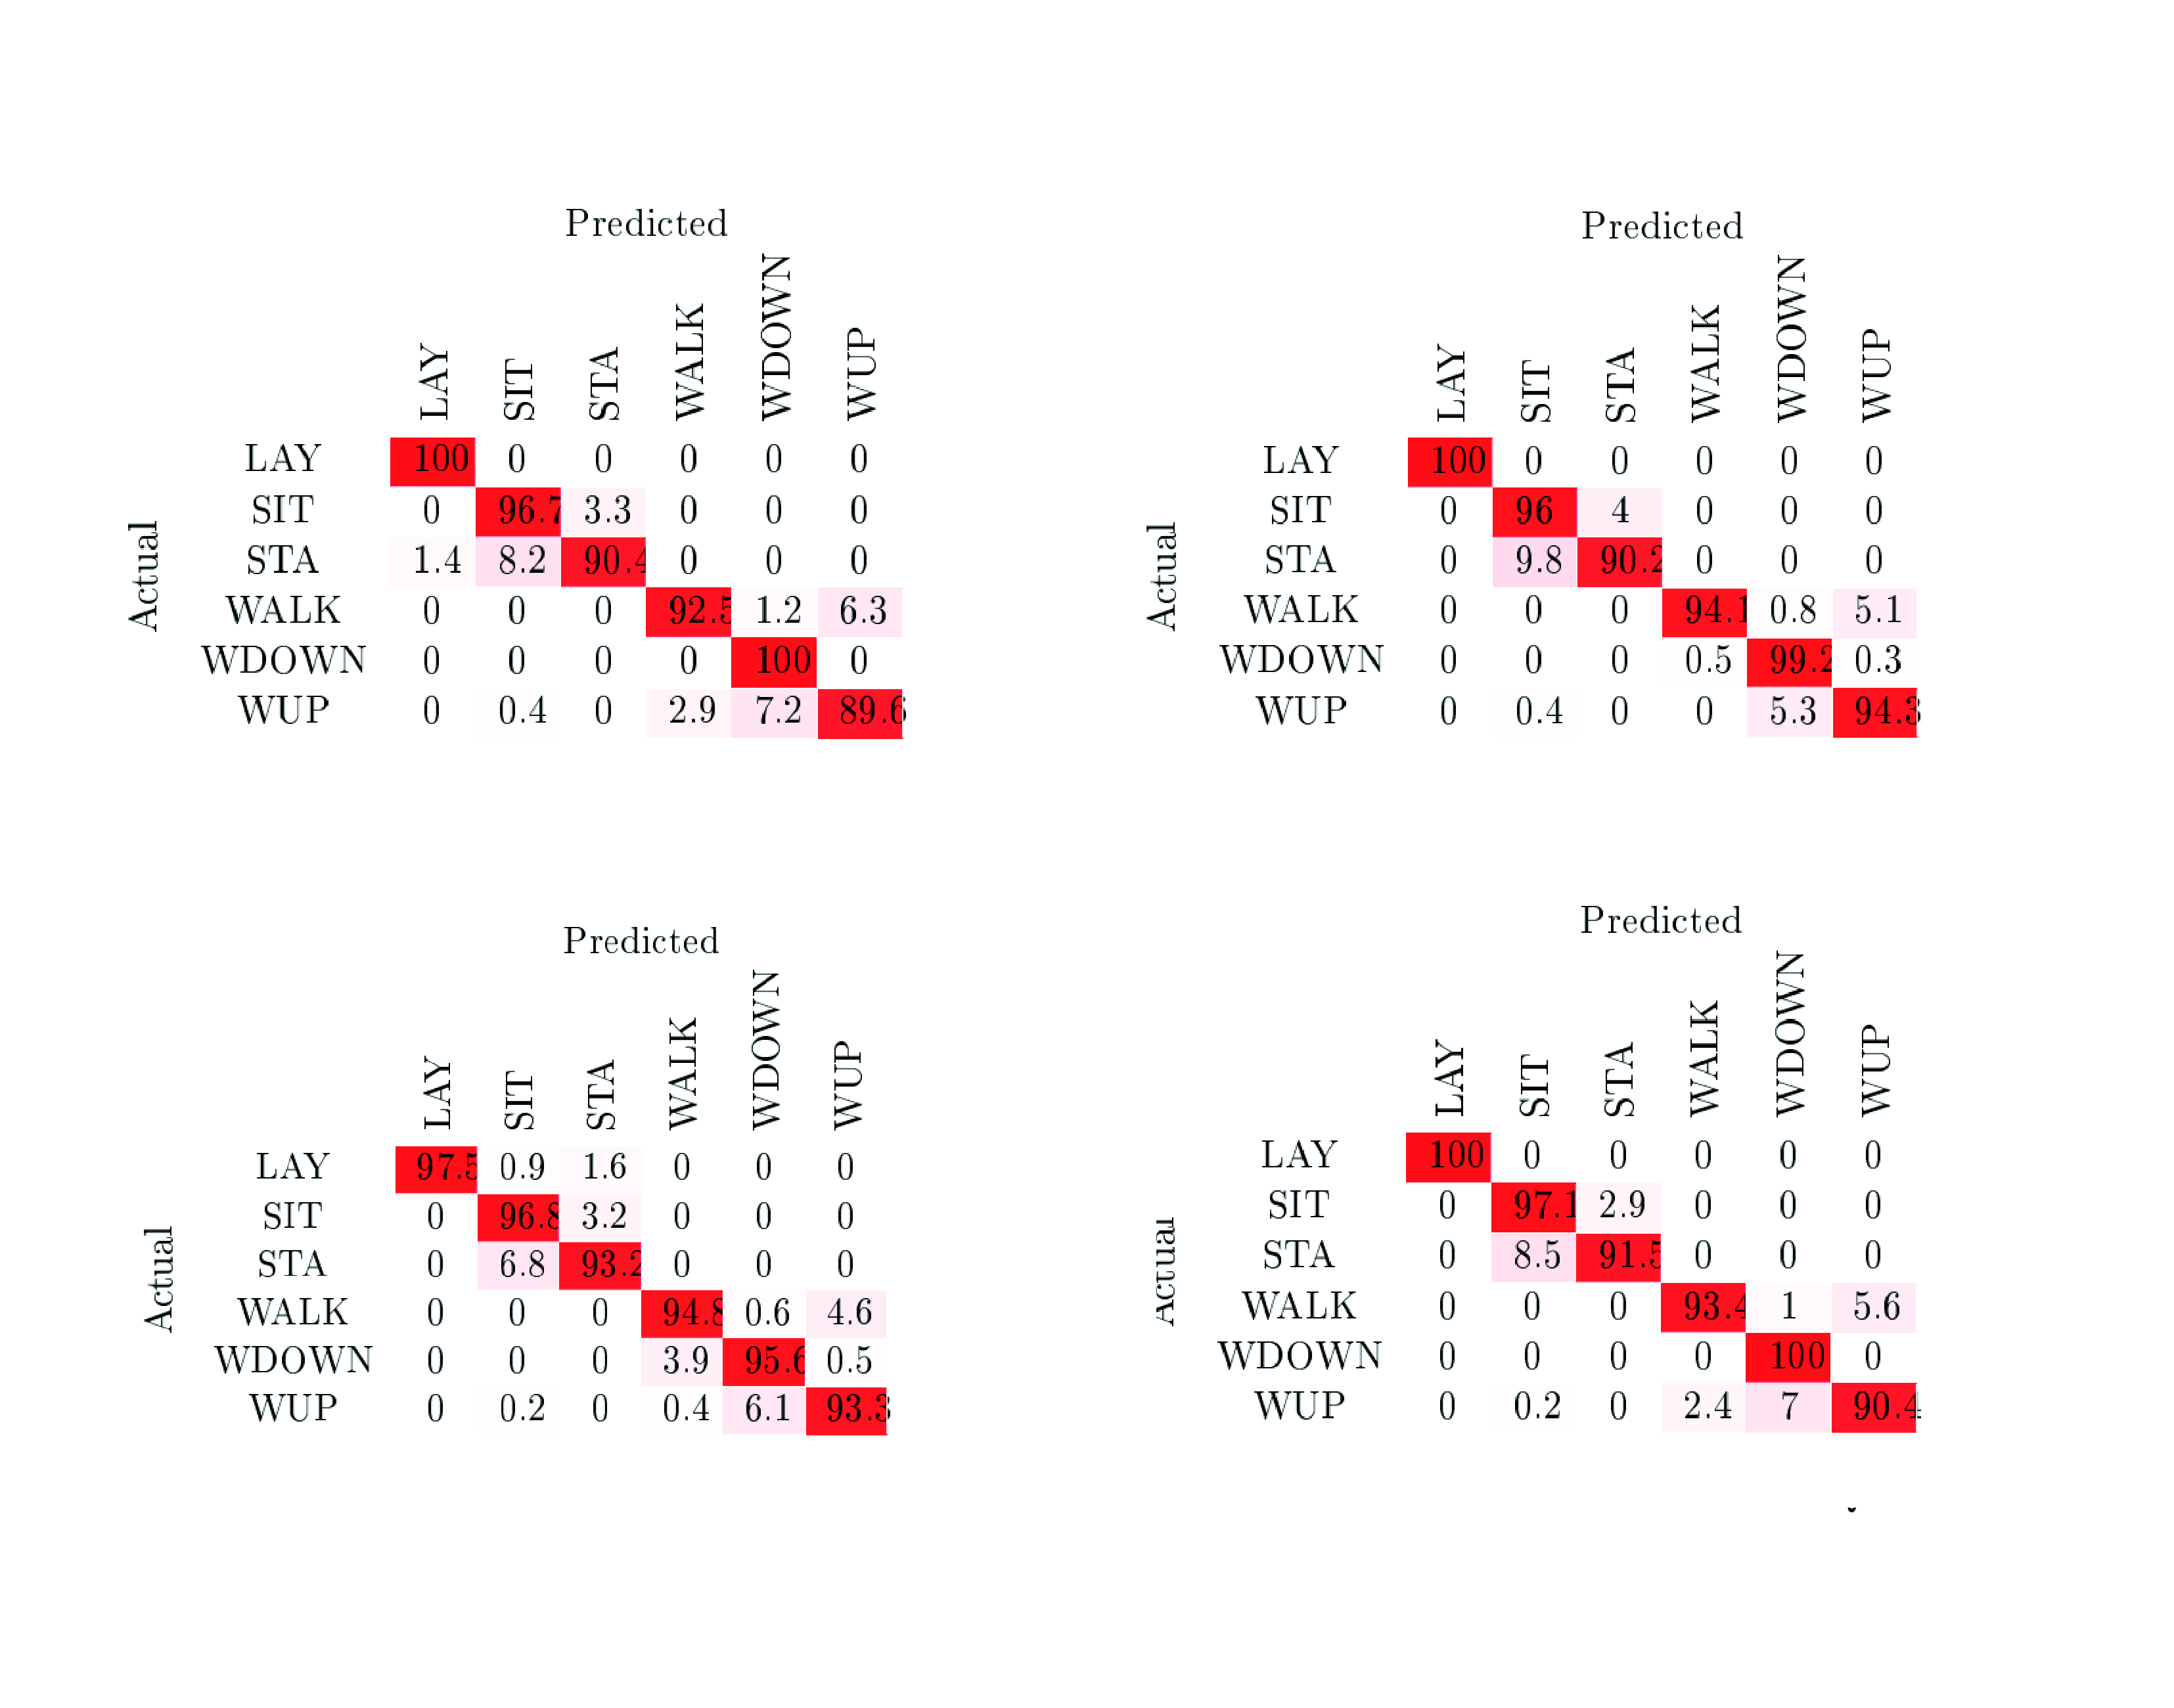
\includegraphics[width=1.0\textwidth]{svm}
\caption{Matrices de confusión para los Kernels de SVM. (a) Cubic (b) Lineal (c) Medium Gaussian (d) Quadratic}
\end{figure}

\begin{figure}[H]
  \centering
    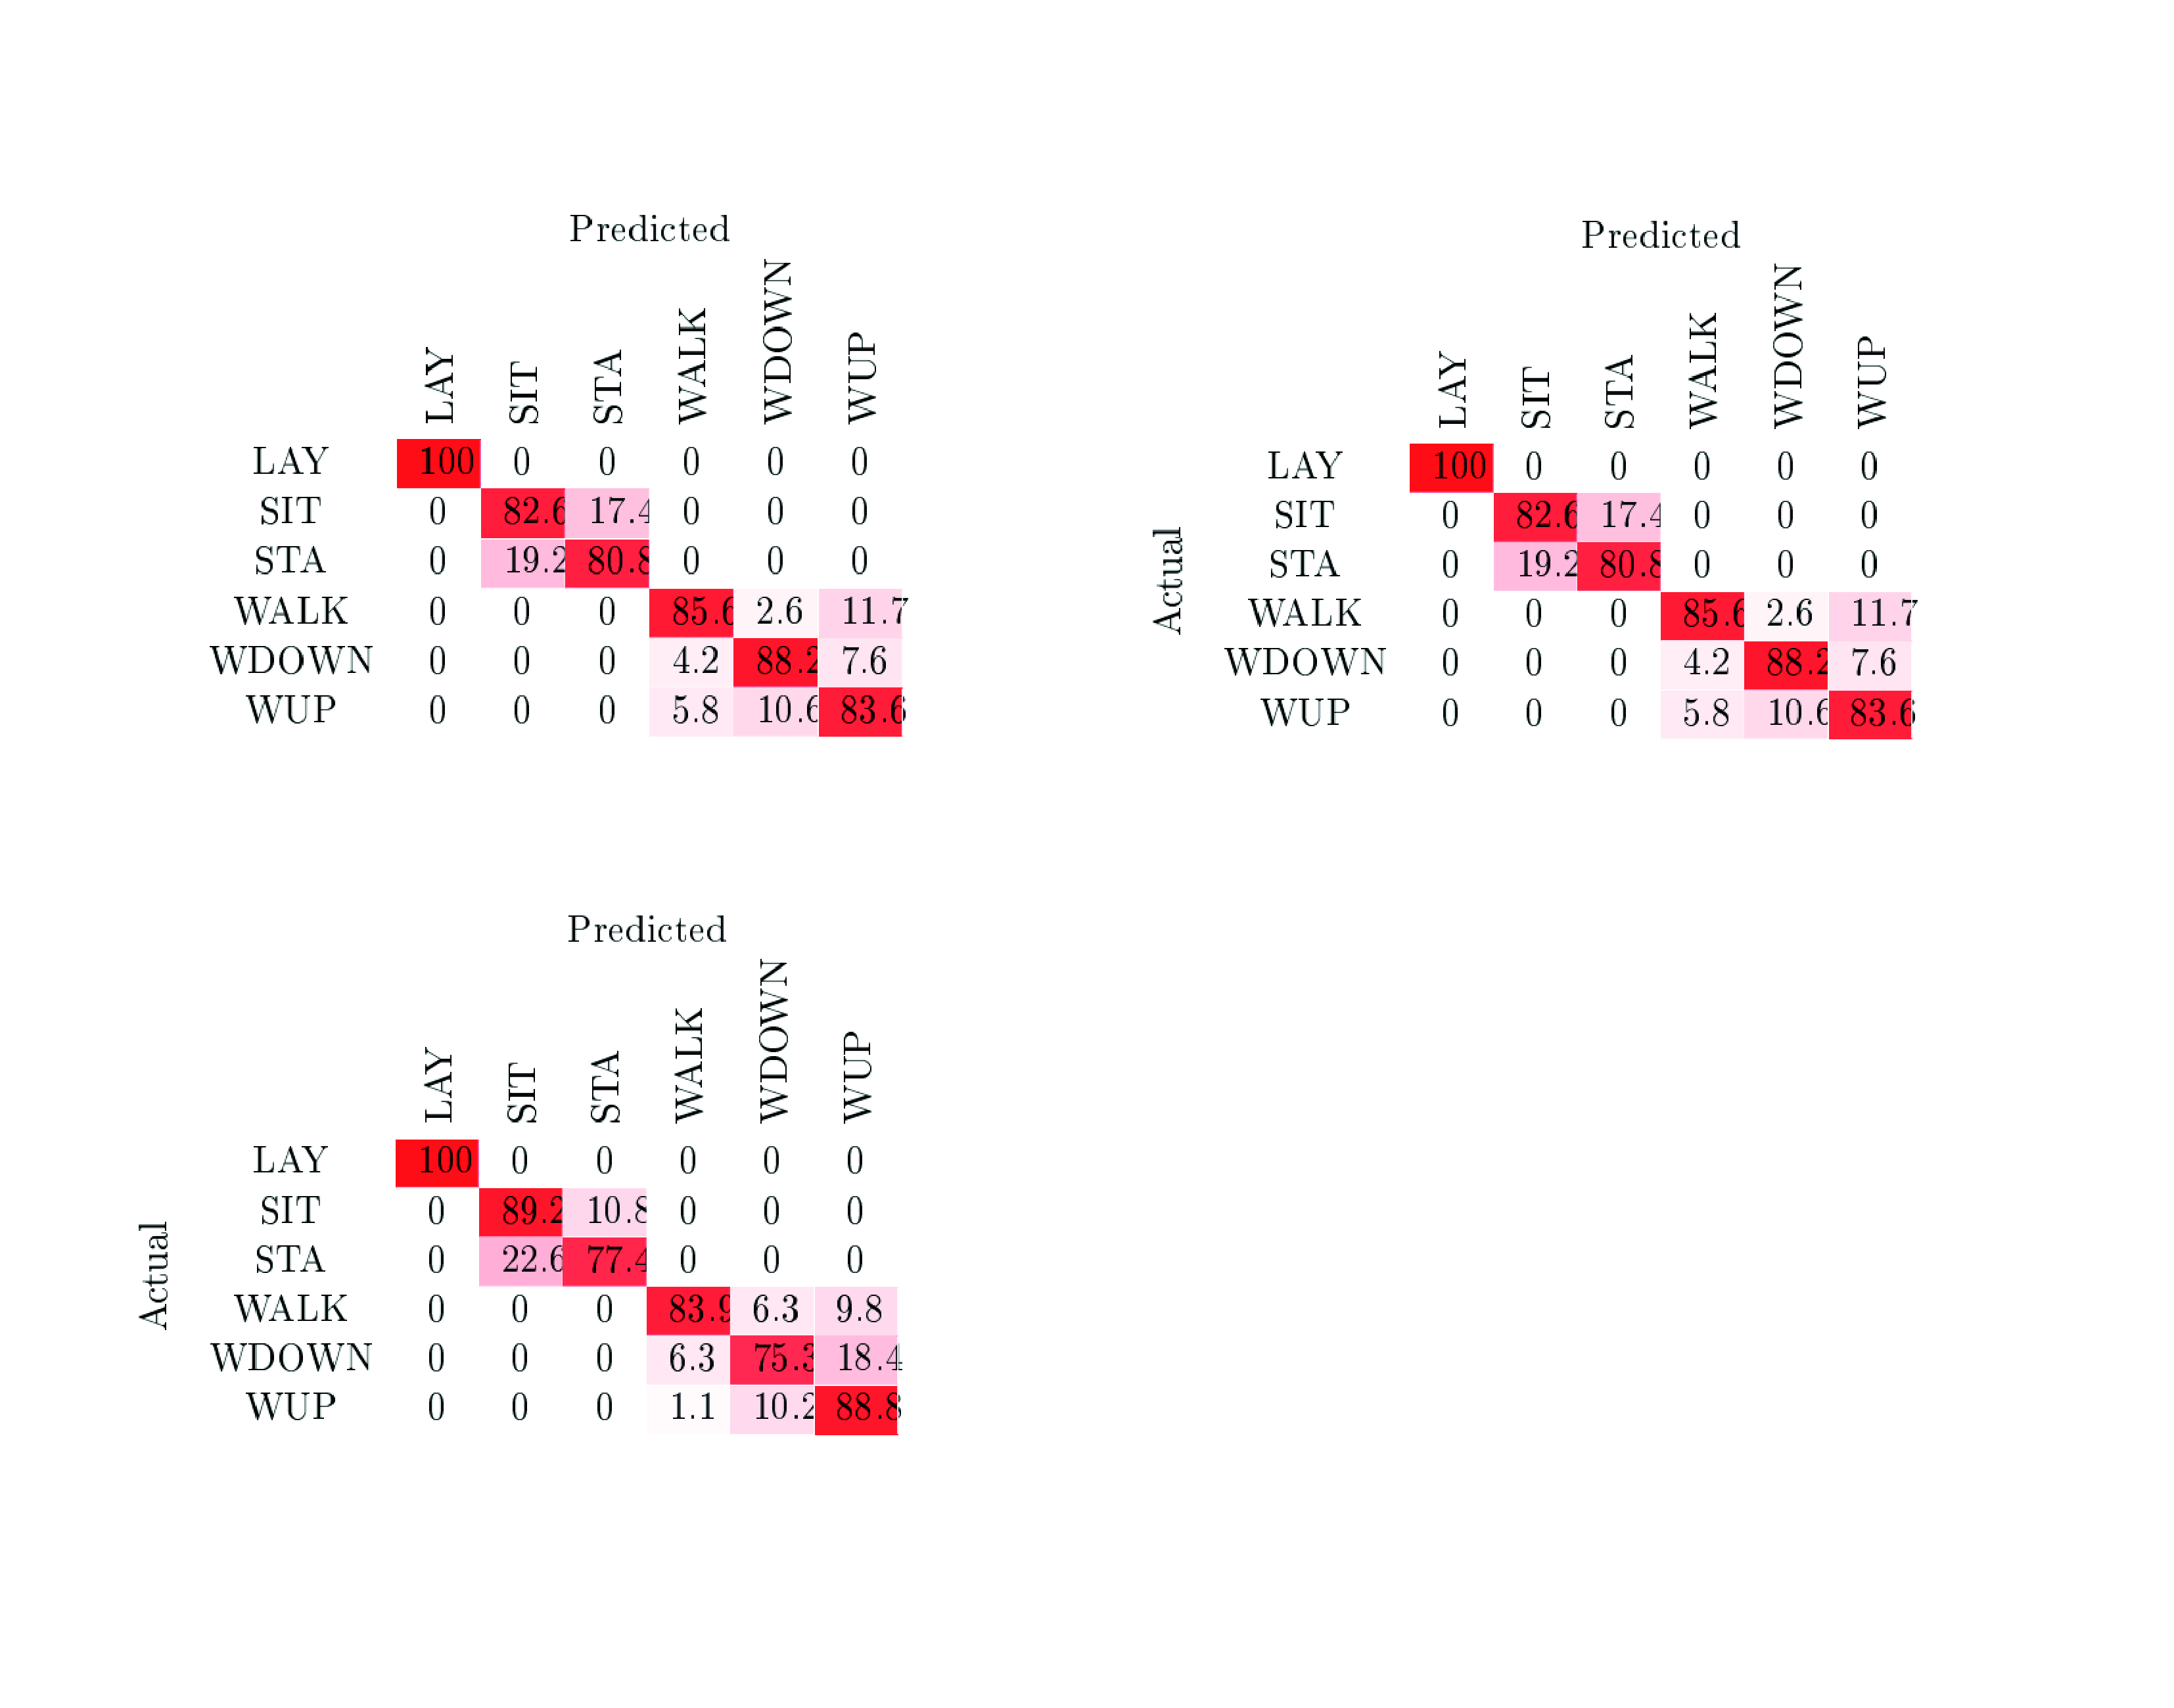
\includegraphics[width=1.0\textwidth]{dt}
\caption{Matrices de confusión para los Kernels de Árbol de decisiones. (a) Simple (b) Complex (c) Medium}
\end{figure}

\begin{figure}[H]
  \centering
    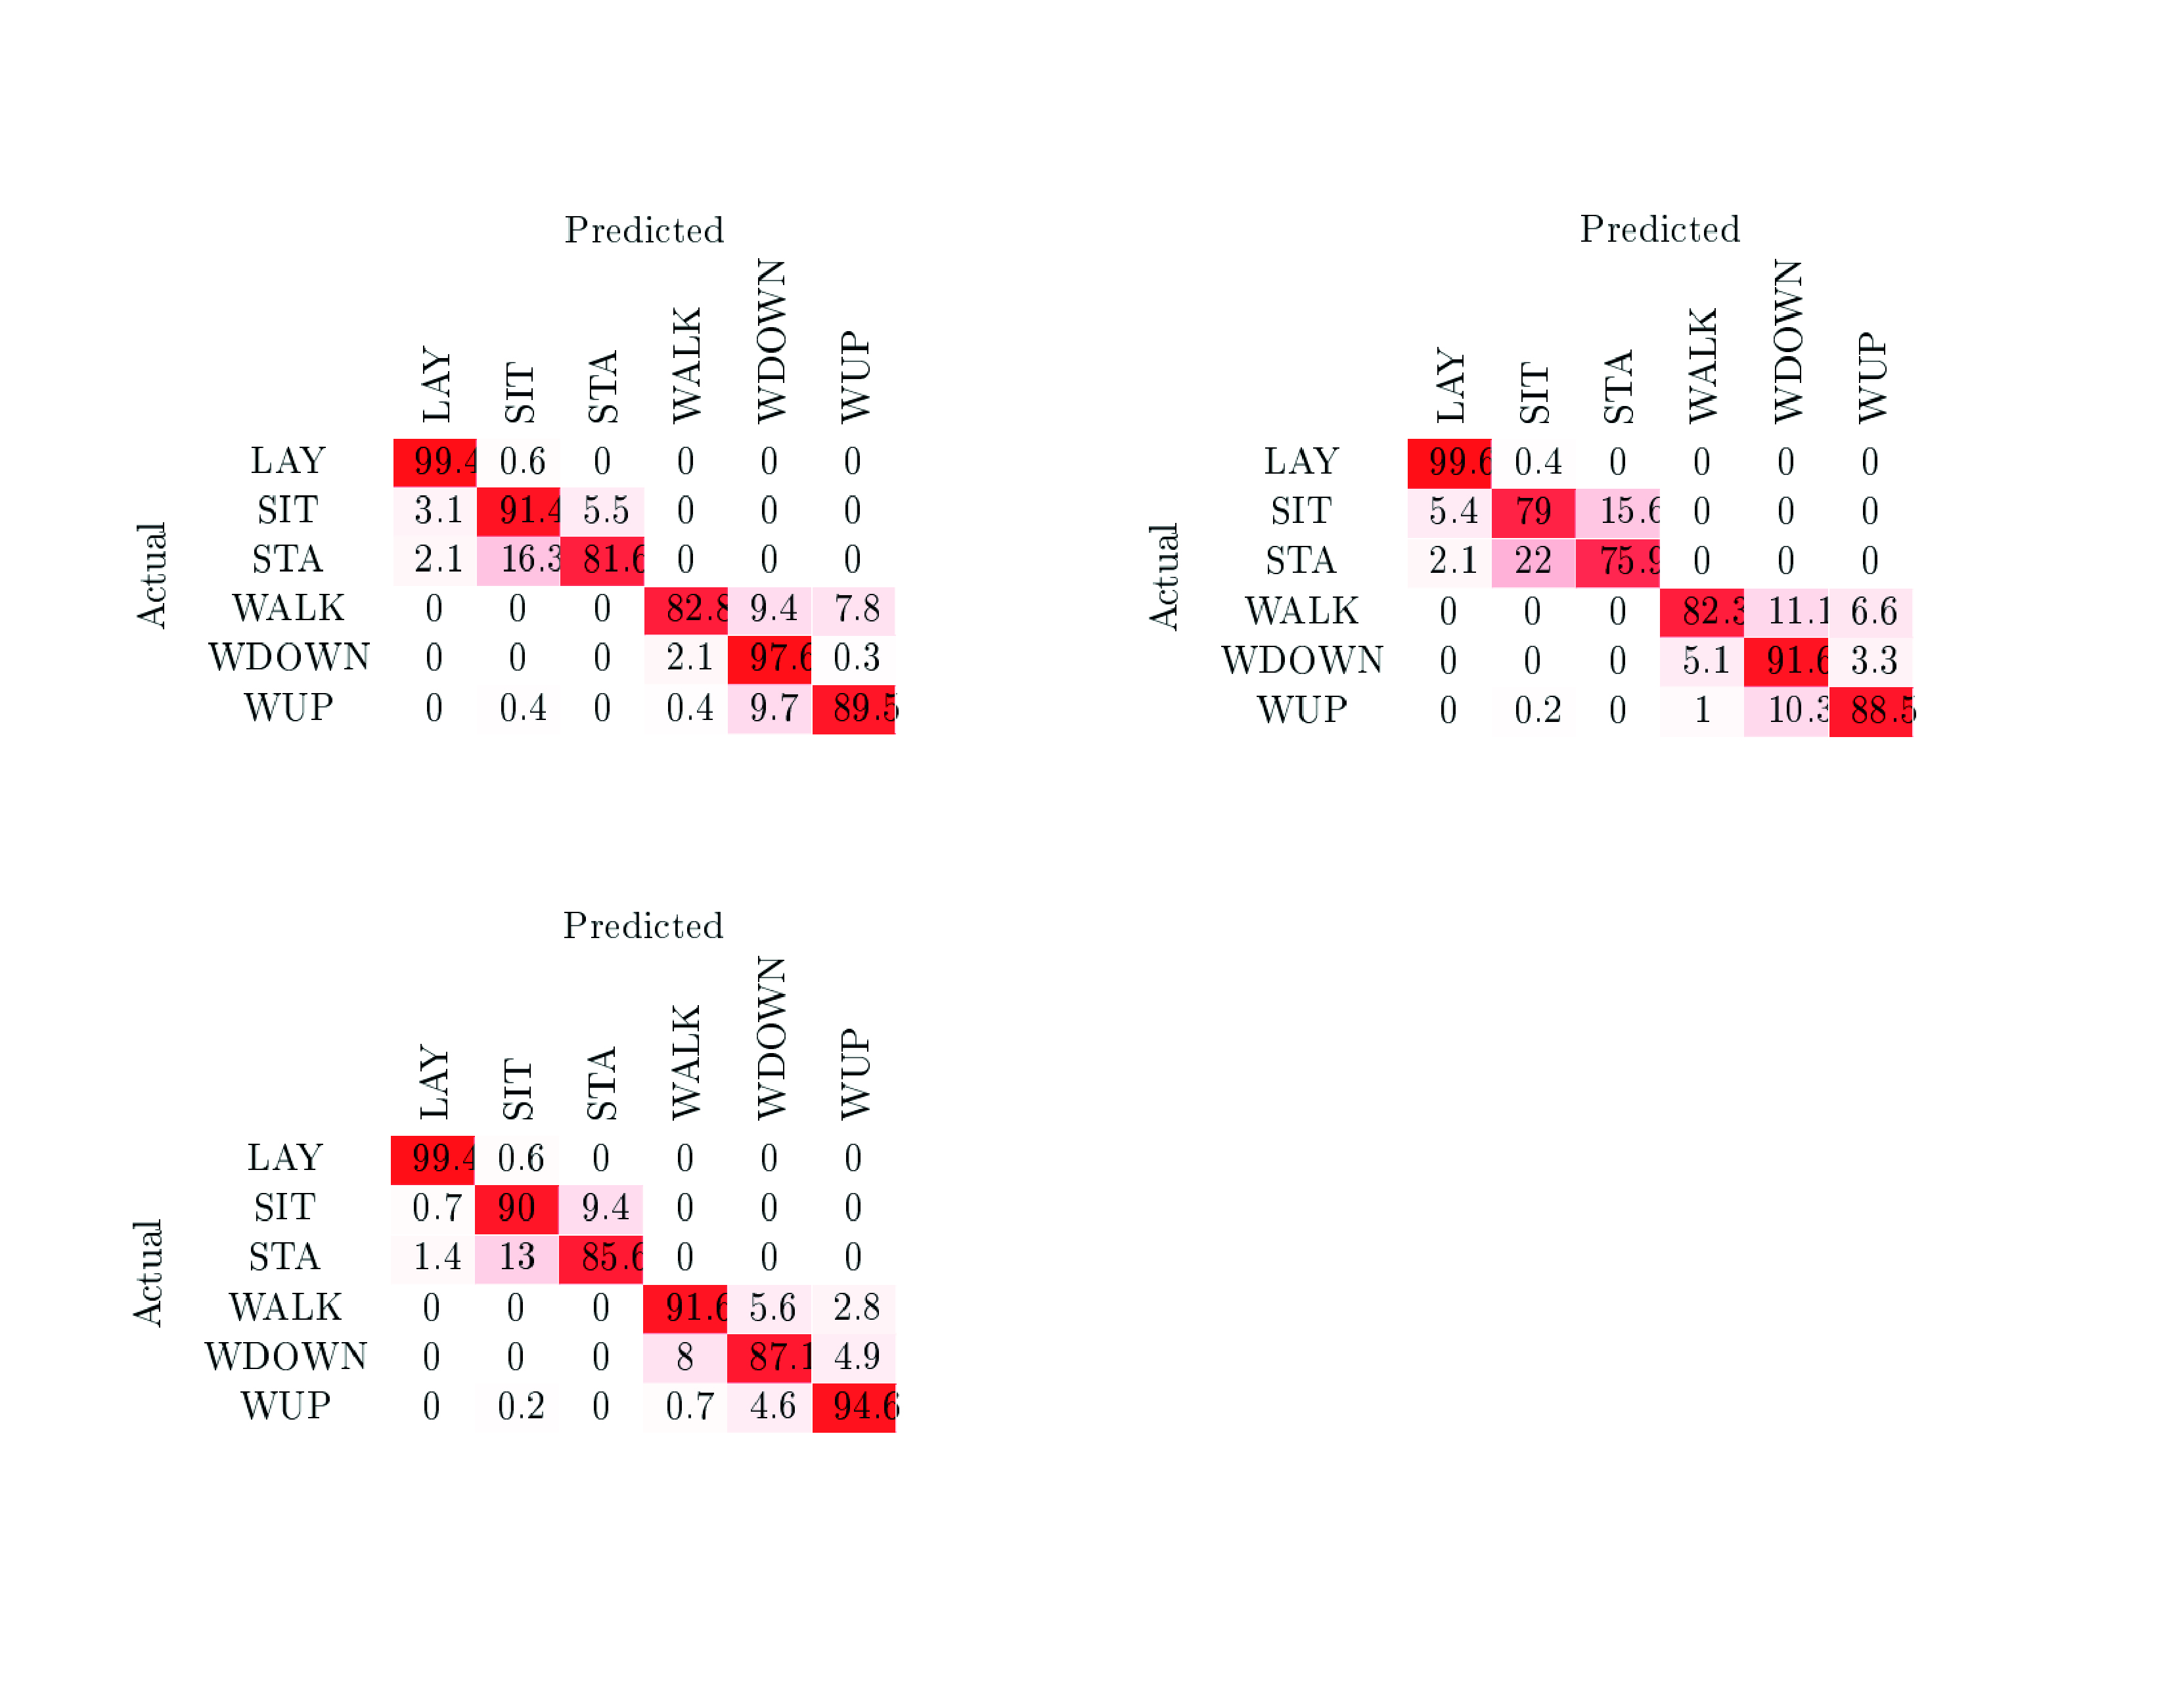
\includegraphics[width=1.0\textwidth]{knn}
\caption{Matrices de confusión para los Kernels de KNN. (a) Weighted (b) Fine (c) Cosine}
\end{figure} 


\section{Protocolo Experimental}

Para realizar la implementación del sensor del Samsung Galaxy SII localizado en dos partes del cuerpo (muñeca y cintura) se realizó el siguiente protocolo de pruebas:

\begin{enumerate}
	\item Consentimiento firmado por la persona a realizar el protocolo (Anexo 1).
	\item Locación del sensor en una de las dos posiciones (muñeca o cintura).
	\item Conexión entre Samsung Galaxy S II y celular auxiliar por medio de TeamViewer.
	\item Ejecución de la acción por parte del voluntario sano. Se monitorea el tiempo de la ejecución por medio de un cronómetro.
	\item Se repiten las 5 acciones restantes.
	\item Se repite el procedimiento para la otra locación del sensor.
	\item Extracción de señales por medio de cable de datos USB.
\end{enumerate}

\par
\medskip
\noindent
Una vez obtenidos los datos de los sensores, se filtró la señal. Los filtros implementados en el pre-procesamiento fueron diseñados en Matlab, con la aplicación 'filter design'. Además, al momento de implementar se utilizó la función 'filtfilt' para obtener cero distorsión de fase. Las especificaciones para el filtro pasabajos de 20 Hz, fueron las siguientes:

\begin{itemize}
\item Filtro pasabajos con método de diseño Butterworth.
\item Filtro de orden 5.
\item Frecuencia de paso 20 Hz y frecuencia de rechazo 25 Hz.
\item Amplitud en la banda de paso 1 dB, Amplitud en la banda de rechazo -60 dB.
\end{itemize}

\par
\medskip
\noindent
El filtro pasabajos para separar la señal de gravedad cumple con las siguientes especificaciones:

\begin{itemize}
\item Filtro pasabajos con método de diseño Butterworth.
\item Filtro de orden 15.
\item Frecuencia de paso 0.3 Hz y frecuencia de rechazo 0.5 Hz.
\item Amplitud en la banda de paso 1 dB, Amplitud en la banda de rechazo -60 dB.
\end{itemize}

\par
\medskip
\noindent
El filtro pasaaltas para separar la señal triaxial correspondiente a los movimientos del cuerpo cumple con las siguientes especificaciones:

\begin{itemize}
\item Filtro pasaaltas con método de diseño Butterworth.
\item Filtro de orden 15.
\item Frecuencia de rechazo 0.3 Hz y frecuencia de paso 0.5 Hz.
\item Amplitud en la banda de paso 1 dB, Amplitud en la banda de rechazo -60 dB.
\end{itemize}

\par
\medskip
\noindent
 La respuesta de los filtros implementados para el preprocesamiento de las señales se observan en las siguientes figuras (4.1, 4.2 y 4.3).

\begin{figure}[H]
 
\begin{subfigure}{1\textwidth}
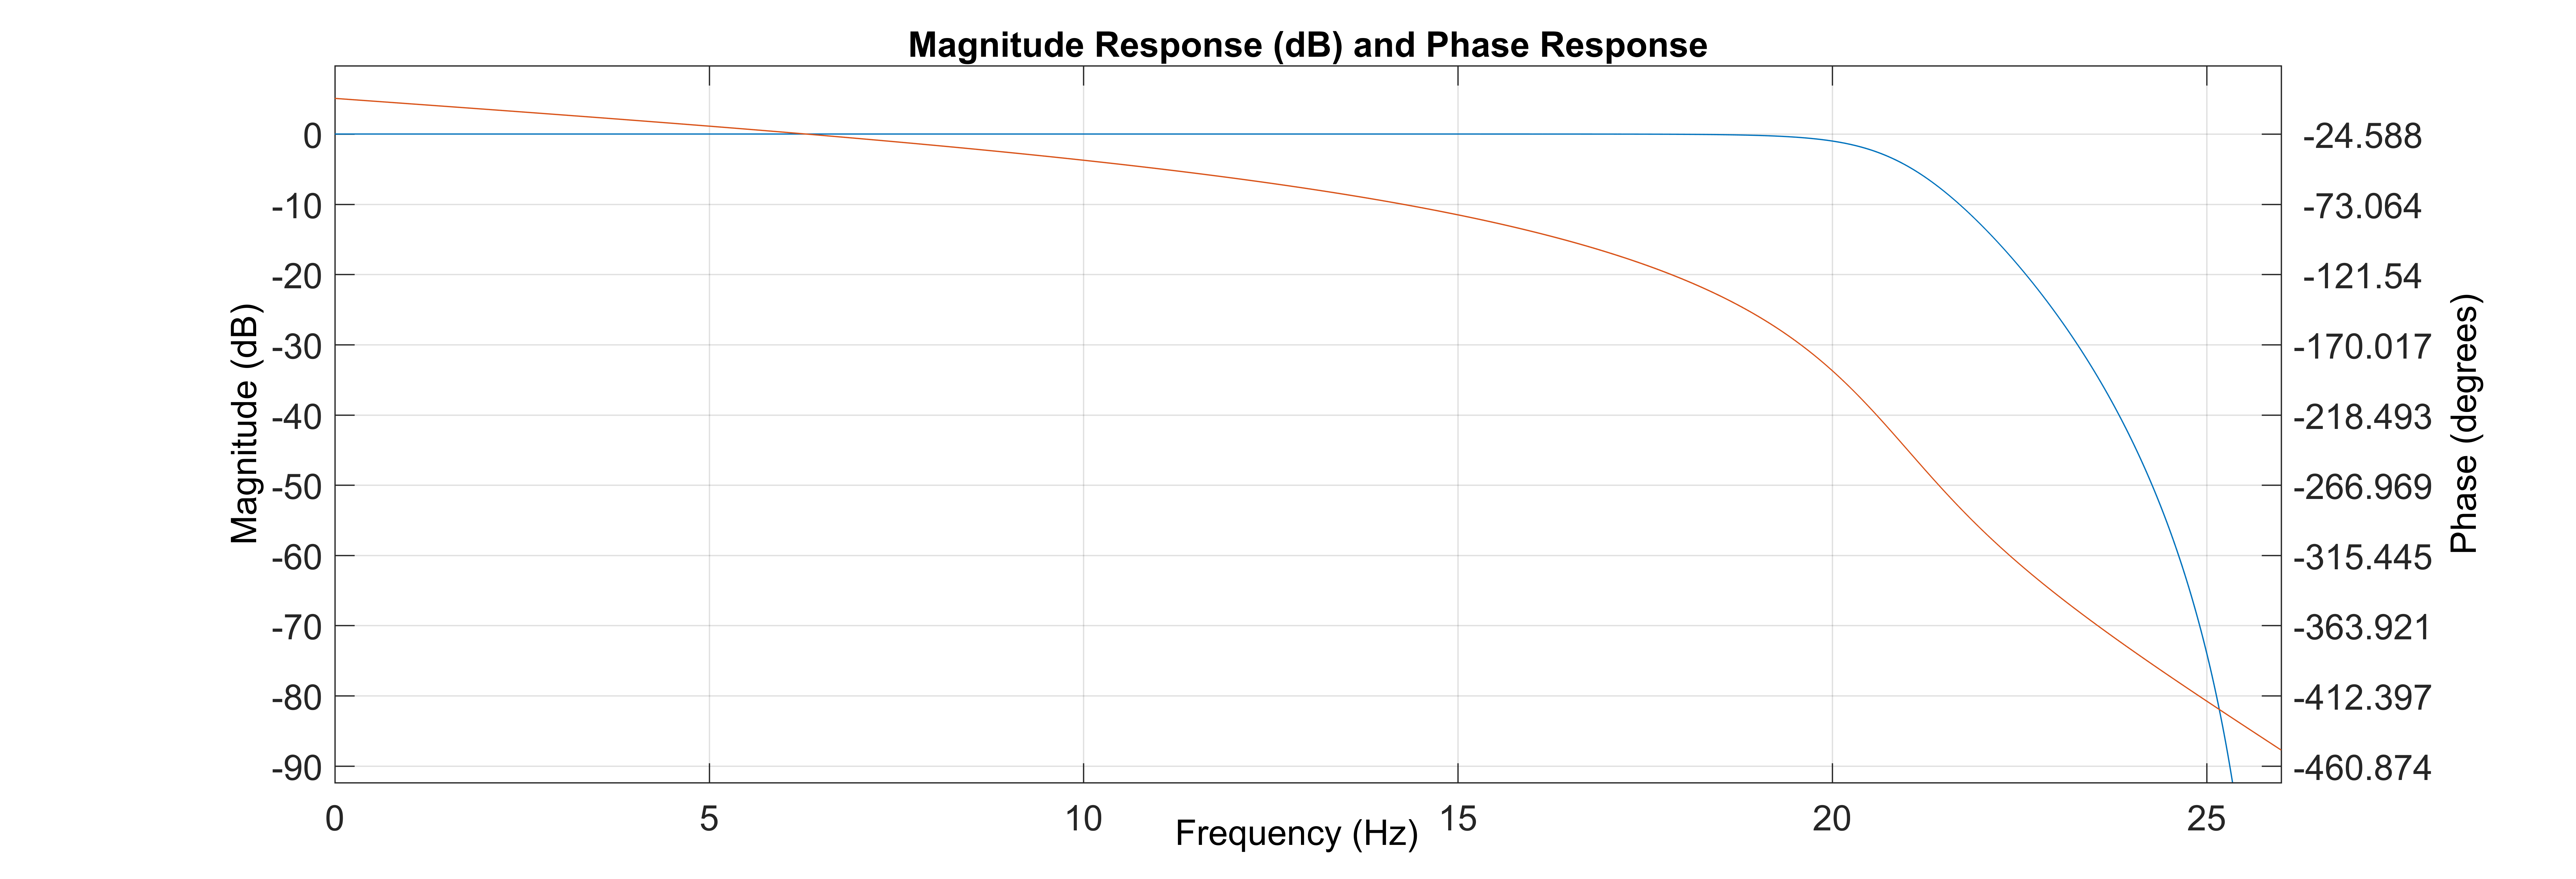
\includegraphics[width=1\linewidth]{filtro_pasabajos20Hz} 
\caption{Respuesta en Frecuencia Filtro Pasabajos 20 Hz}
\label{fig:subim1}
\end{subfigure}
\begin{subfigure}{1\textwidth}
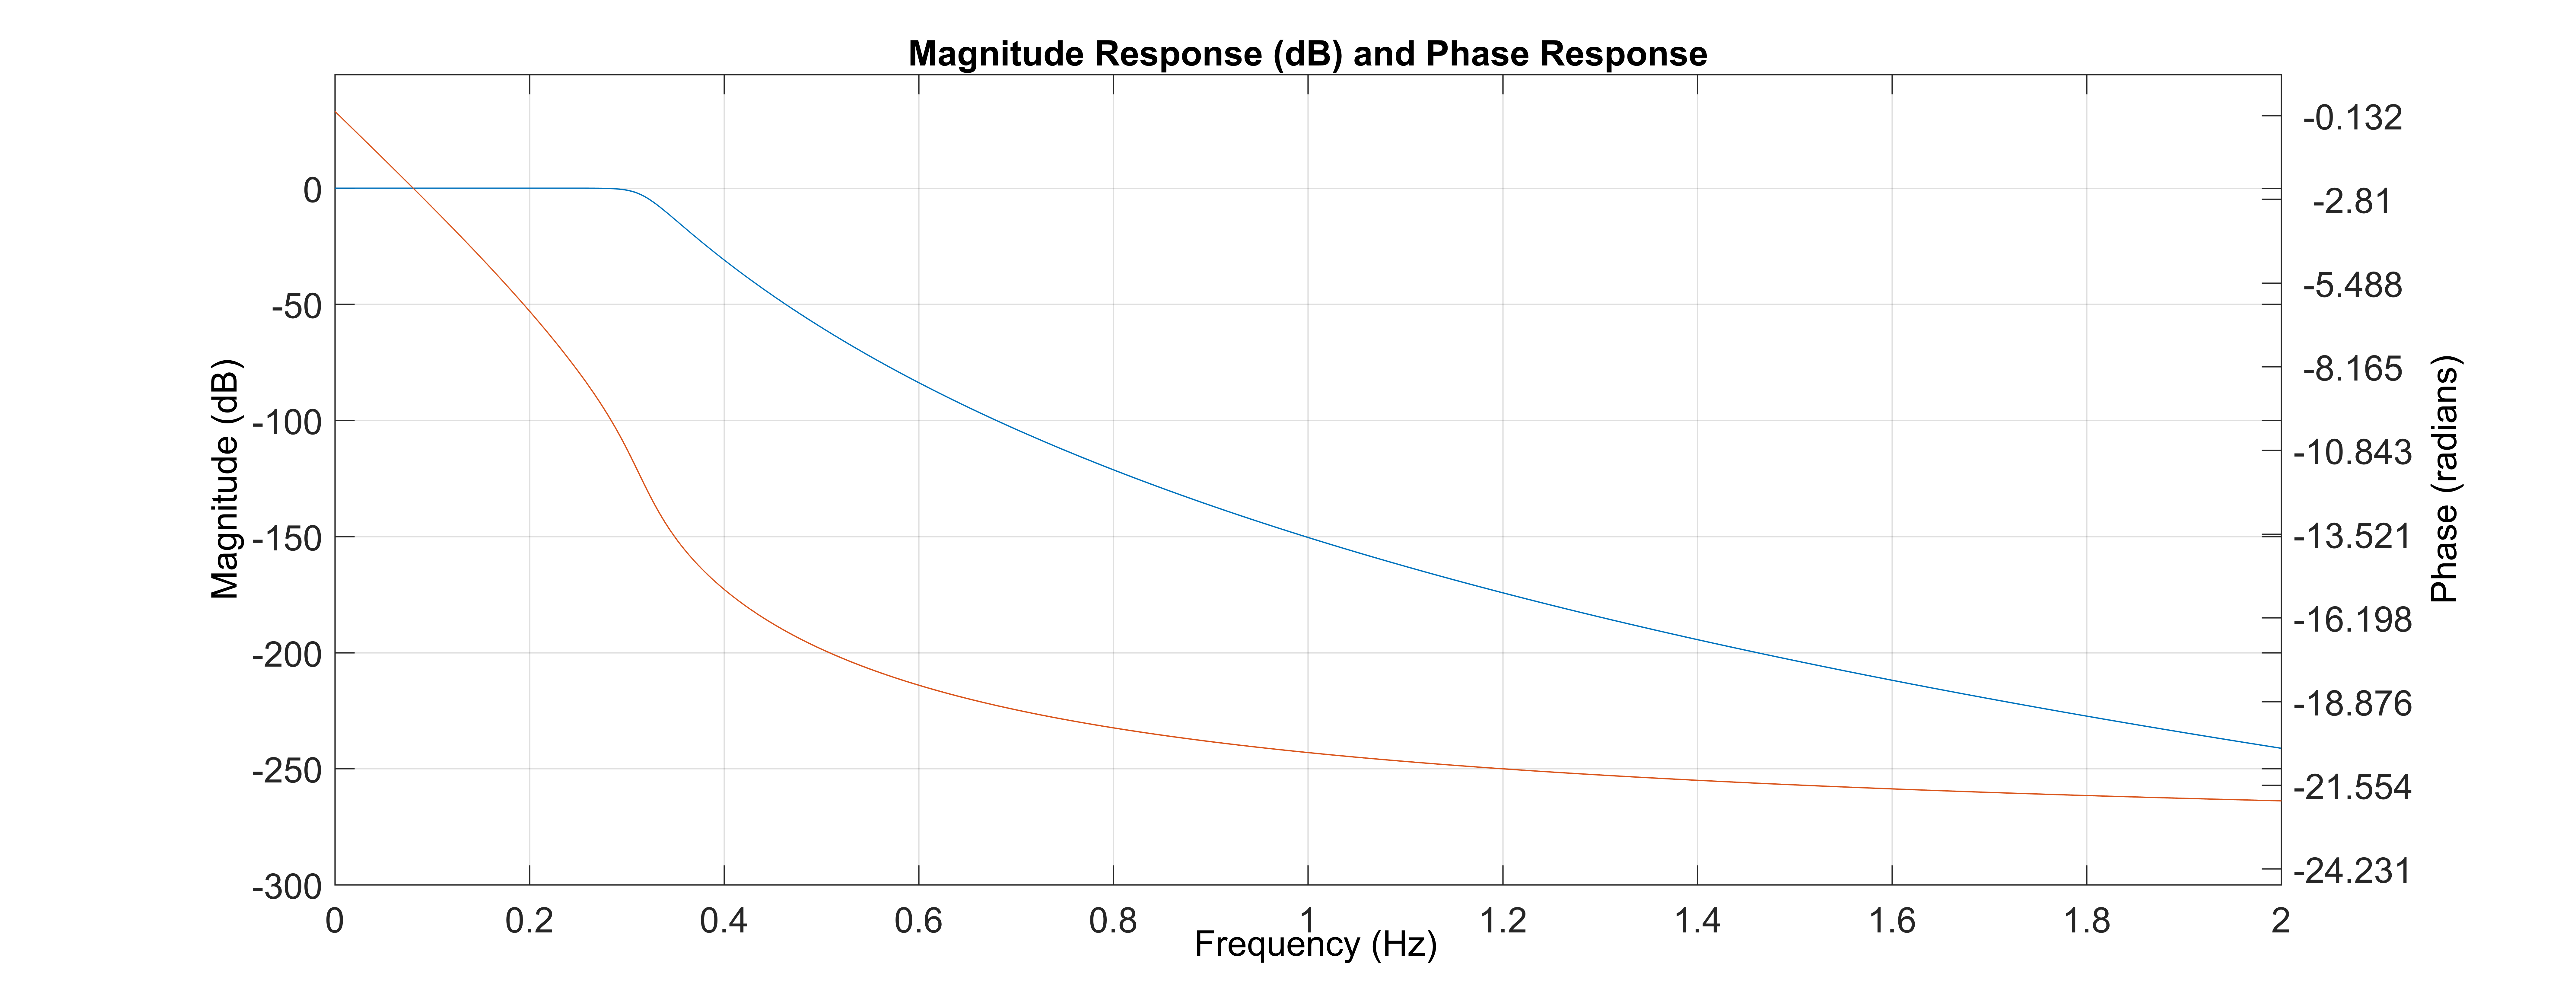
\includegraphics[width=1\linewidth]{filtro_pasabajos0_3Hz}
\caption{Respuesta en Frecuencia Filtro Pasabajos 0.3 Hz}
\label{fig:subim2}
\end{subfigure}
 \begin{subfigure}{1\textwidth}
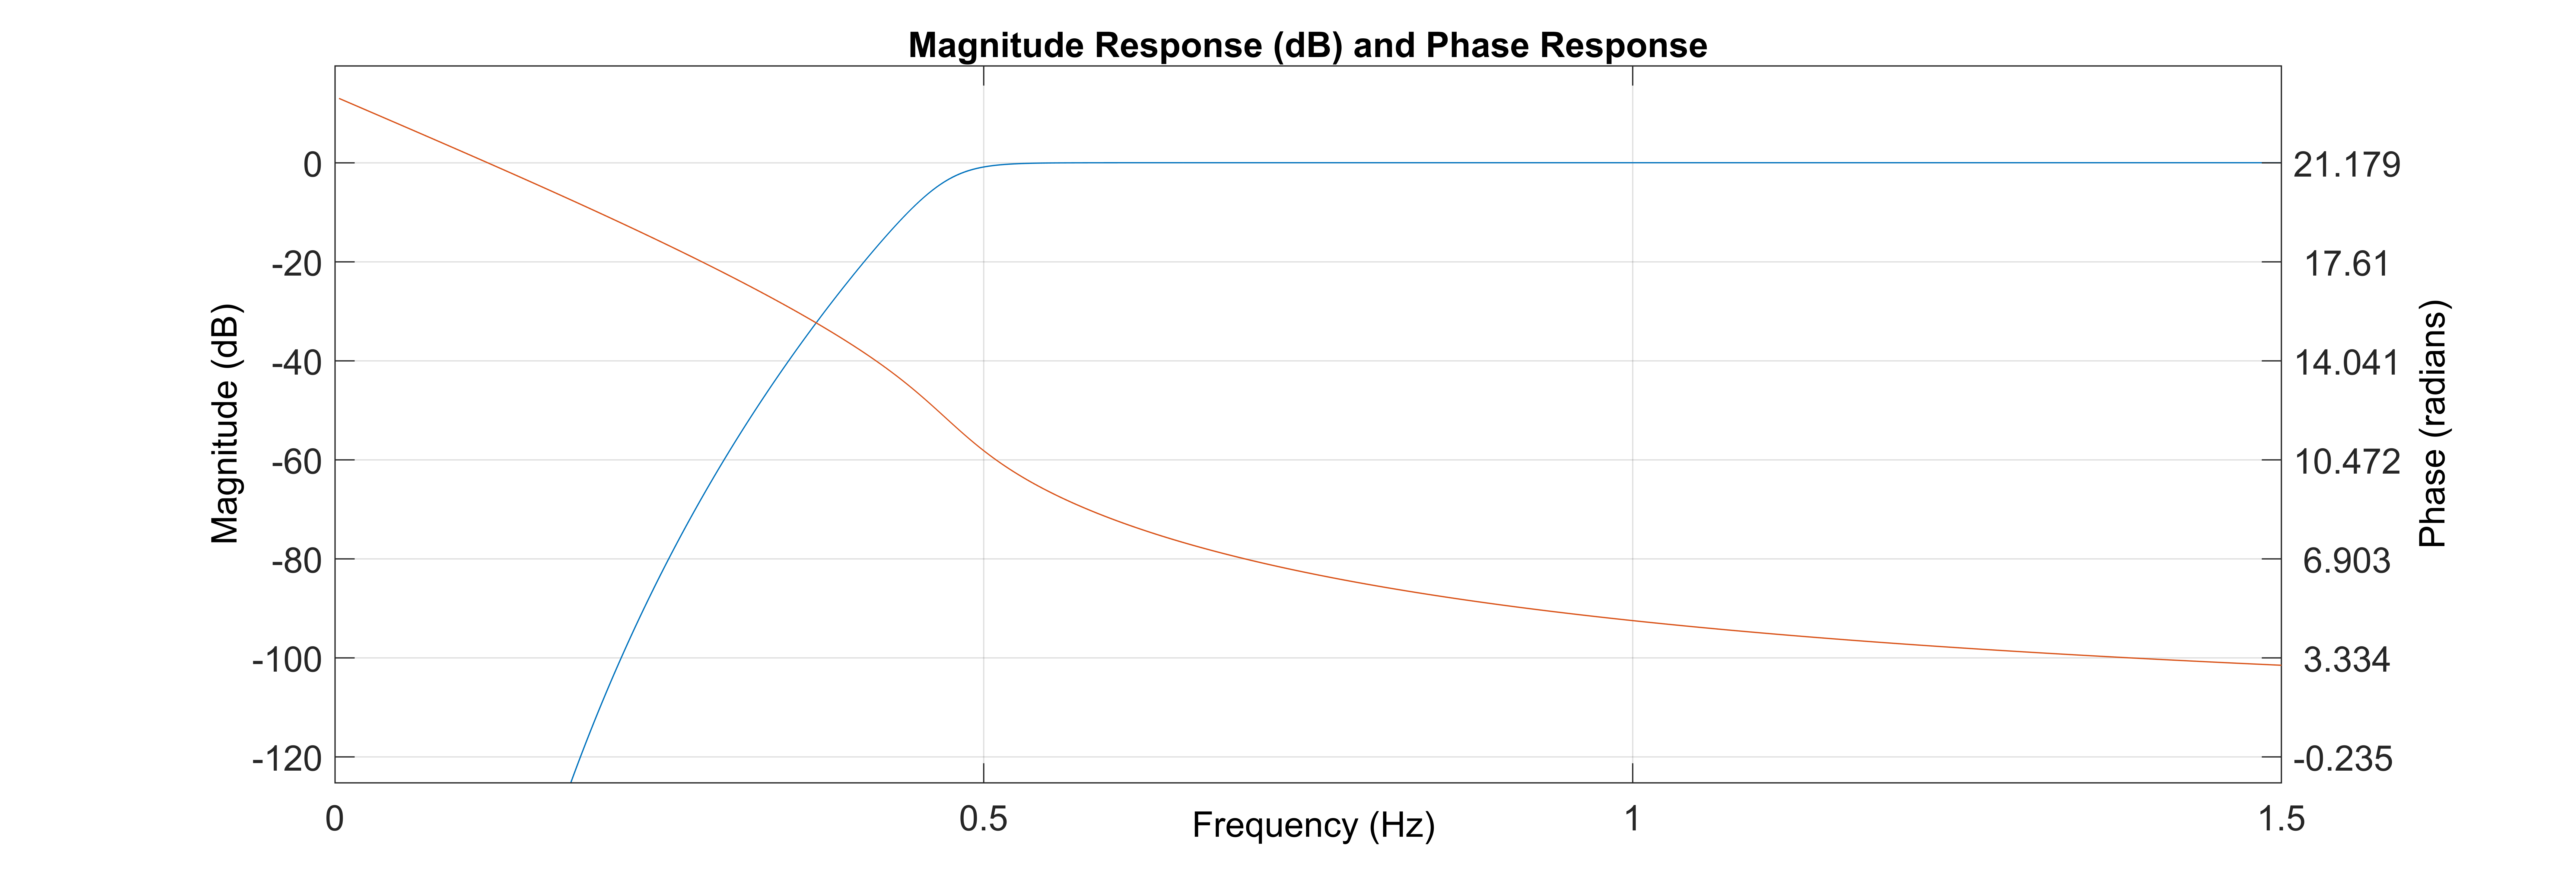
\includegraphics[width=1\linewidth]{pasaaltas0_5Hz}
\caption{Respuesta en Frecuencia Filtro Pasaaltos 0.5 Hz}
\label{fig:subim3}
\end{subfigure}

\caption{Respuesta en Frecuencia de los Filtros implementados}
\label{fig:image2}
\end{figure}


 \begin{figure}[H]
  \centering
    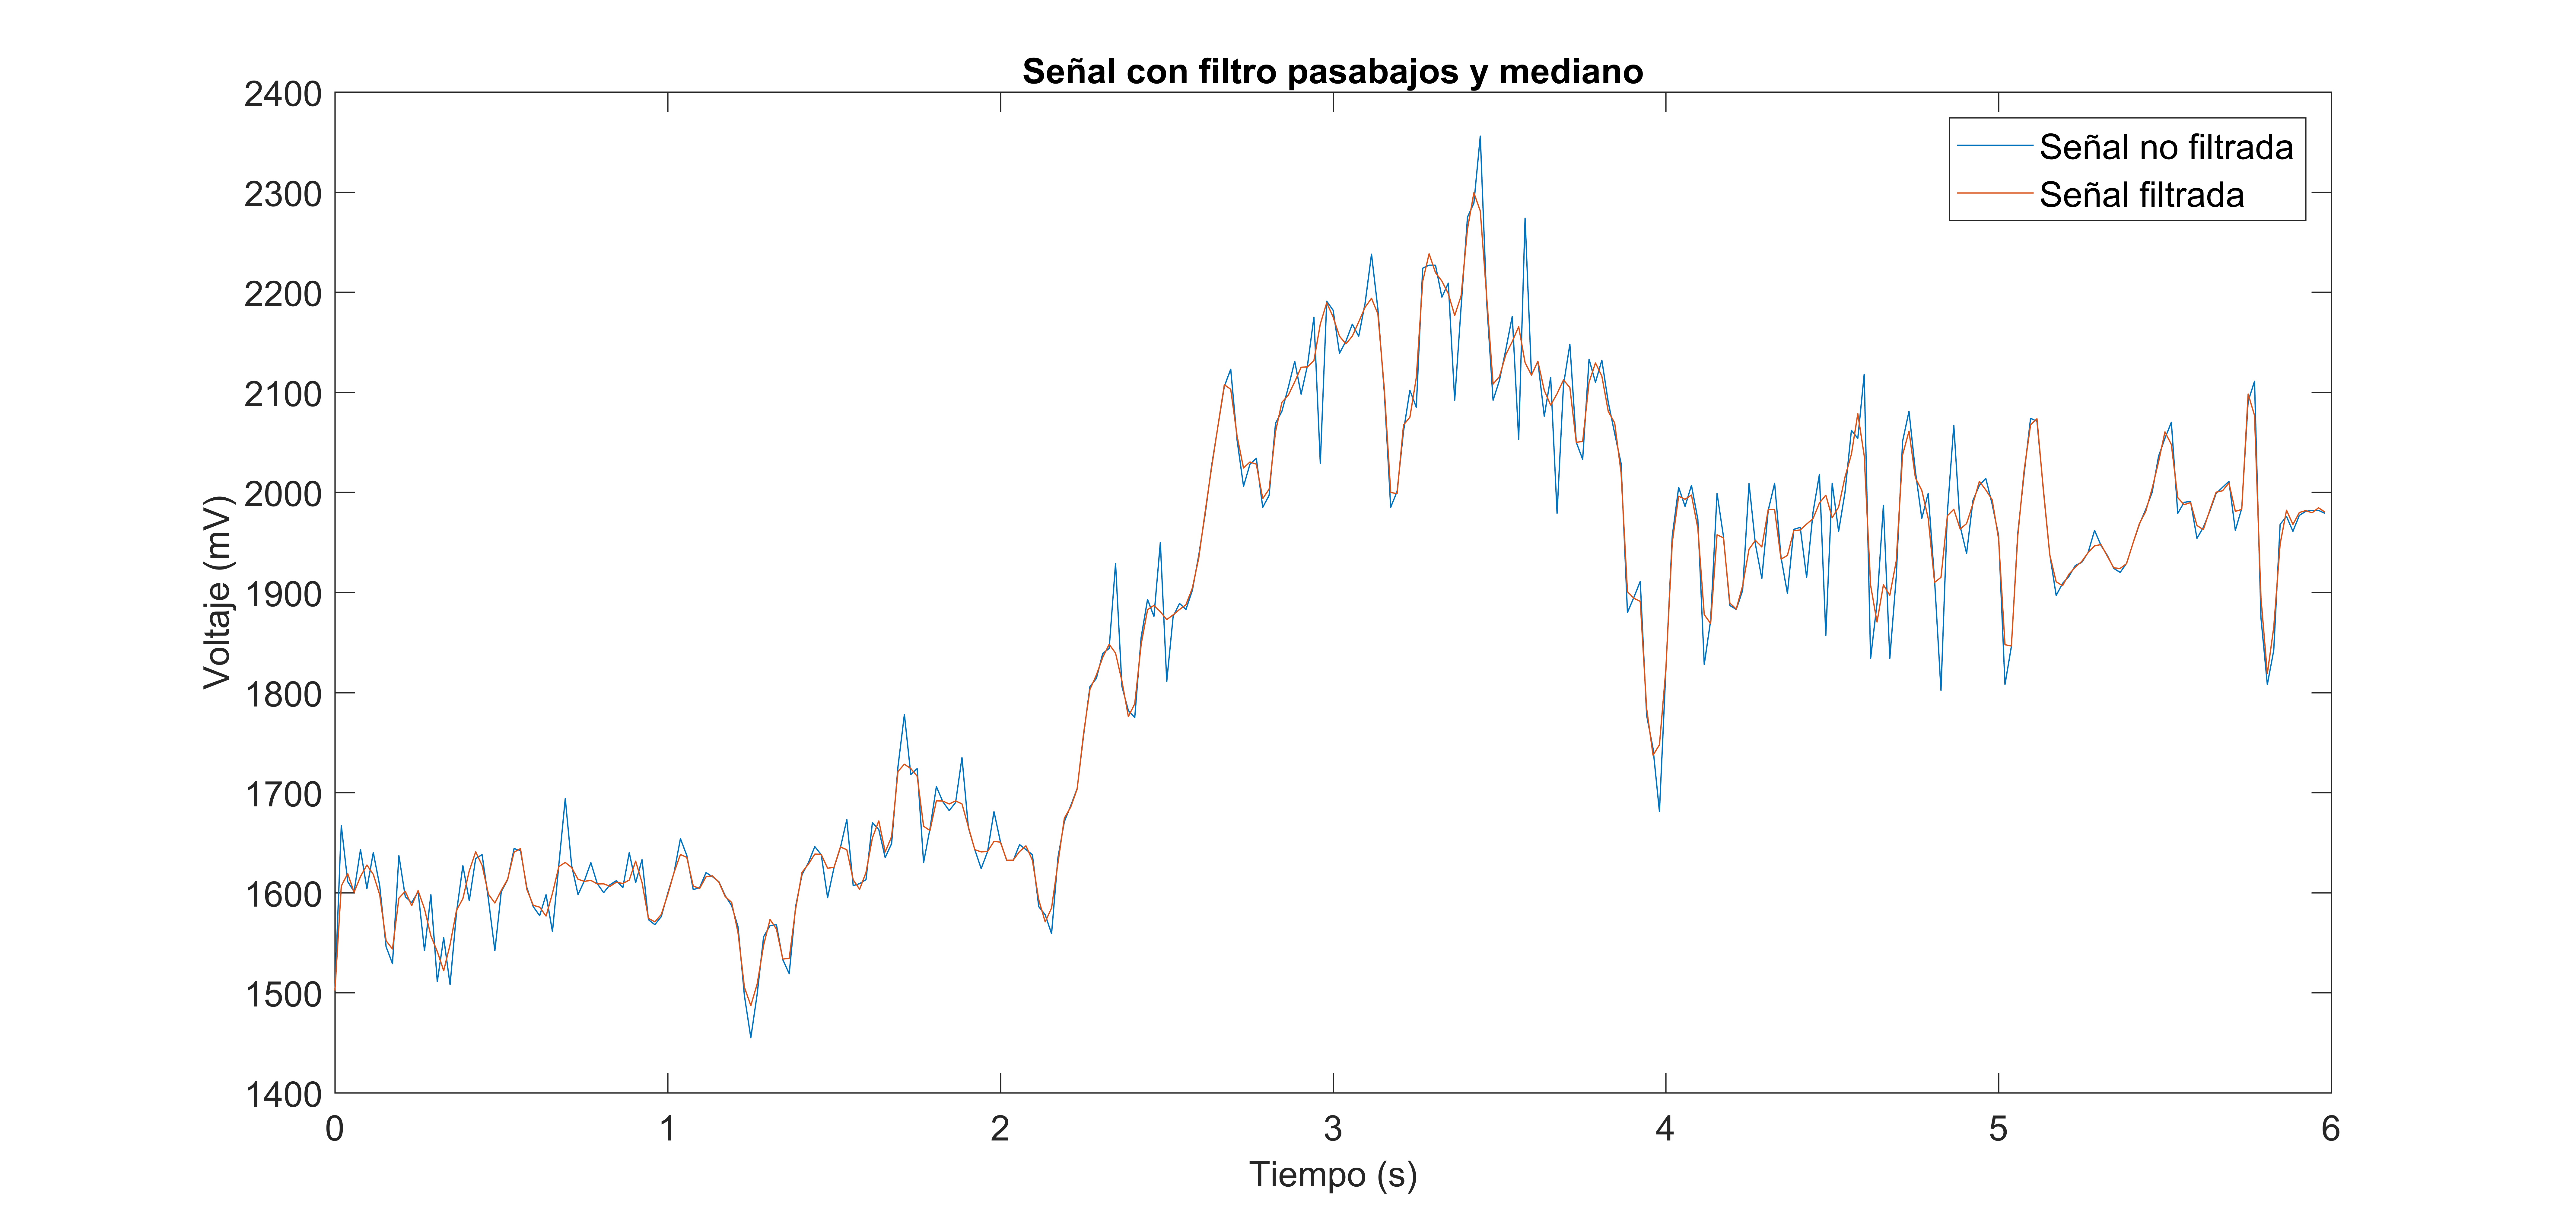
\includegraphics[width=1\textwidth]{senal_filtrada}
   \caption{Respuesta en tiempo Señal Filtrada (Eje X del acelerómetro)}
  \end{figure}

 \begin{figure}[H]
  \centering
    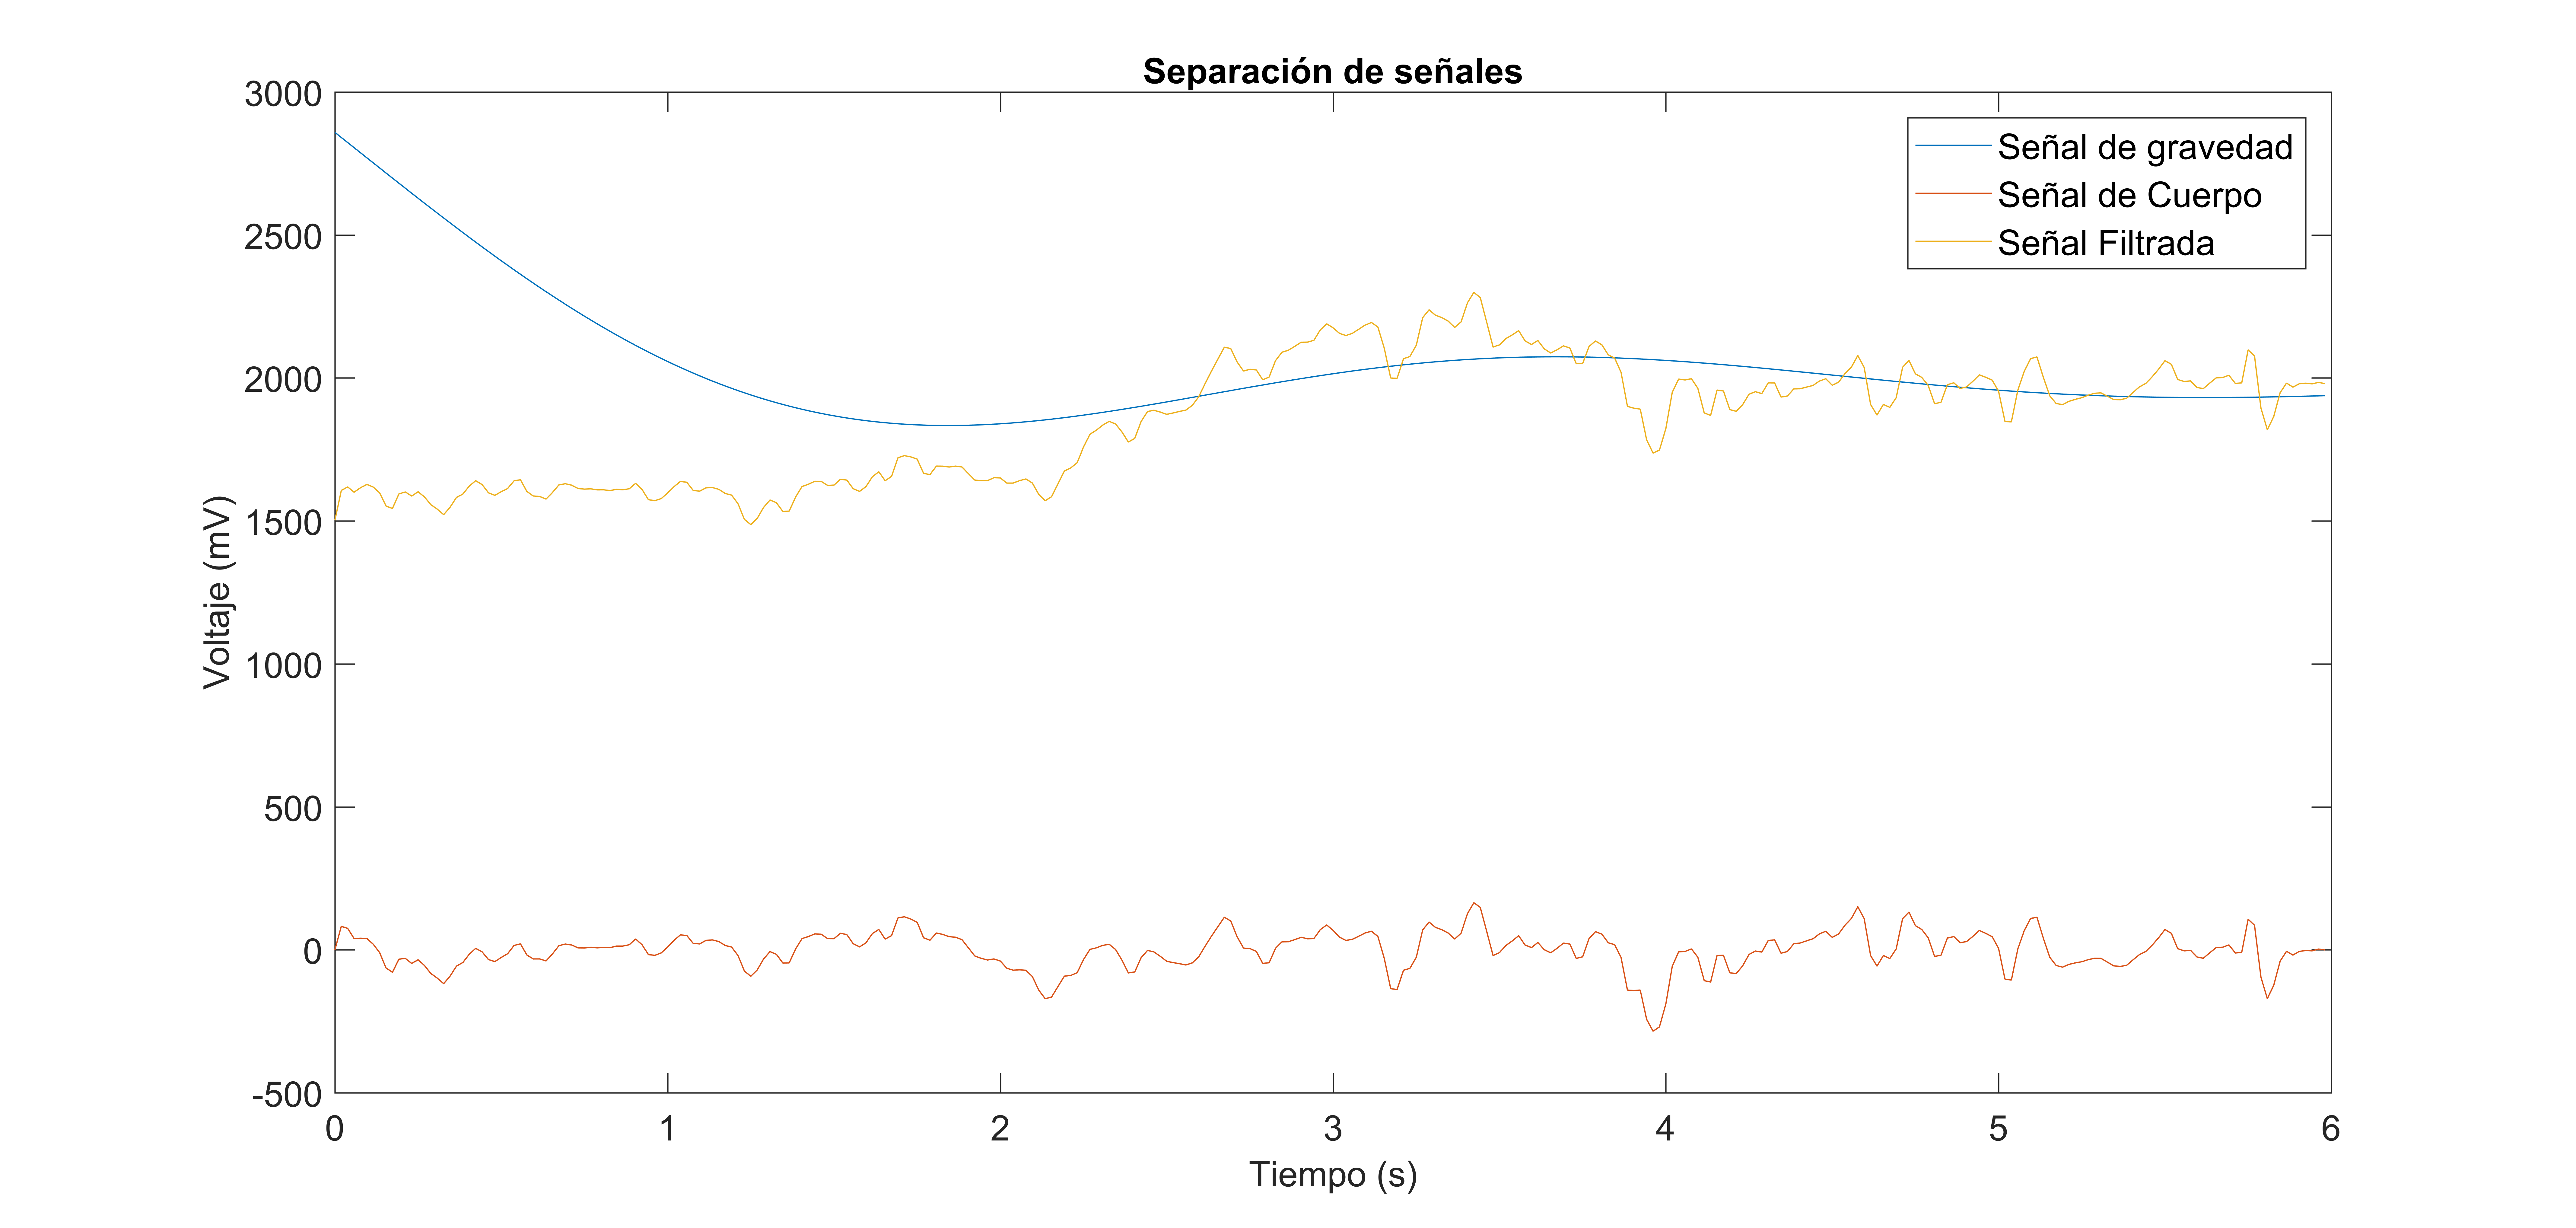
\includegraphics[width=1\textwidth]{senal_separada}
   \caption{Respuesta en tiempo Señal Separada}
  \end{figure}


\par
\medskip
\noindent

En cuanto a la selección de características, se segmentaron las señales en tiempo y frecuencia y se obtuvieron los siguientes vectores:

\begin{itemize}
\item Acelerómetro Cuerpo tiempo.
\item Acelerómetro Gravedad tiempo.
\item Acelerómetro Cuerpo Jerk tiempo.
\item Giroscopio Cuerpo tiempo.
\item Giroscopio Cuerpo Jerk tiempo.
\item Magnitud (Acelerómetro Cuerpo tiempo).
\item Magnitud (Acelerómetro Gravedad tiempo).
\item Magnitud (Acelerómetro Cuerpo Jerk tiempo).
\item Magnitud (Giroscopio Cuerpo tiempo).
\item Magnitud (Giroscopio Cuerpo Jerk tiempo).
\end{itemize}

Una vez los vectores son calculados, se implementan dos funciones, una para obtener las características en tiempo y otra para obtener las características en frecuencia de cada uno de los vectores. Estas funciones dividen el vector por ventanas como se mencionó en el procesamiento de señales y calcula las características para cada ventana. Estas características se van añadiendo a la base de datos final, la cual va a ser entrenada. El costo computacional para importar los datos a matlab e implementar la extracción de características para 21 personas, se presenta a continuación:

\begin{itemize}
\item Tiempo importando los datos: 3 segundos.
\item Tiempo de filtrado y separación de los vectores: 7 minutos, 8 segundos.
\item Tiempo de extracción de características: 19 minutos, 25 segundos.
\end{itemize}

\chapter{ANÁLISIS DE RESULTADOS}

\section{Análisis de Características}

Para poder observar las características más discriminatorias en el proceso de clasificación, fue calculada la varianza de cada una de las características en la base de datos de train y se escogieron las 8 características de mayor varianza y para cada una de estas características se realizó un boxplot (es un gráfico basado en cuartiles mediante el cual se visualiza la distribución de un conjunto de datos \cite{boxplot}) y los resultados son los siguientes:

\begin{figure}[H]
  \centering
    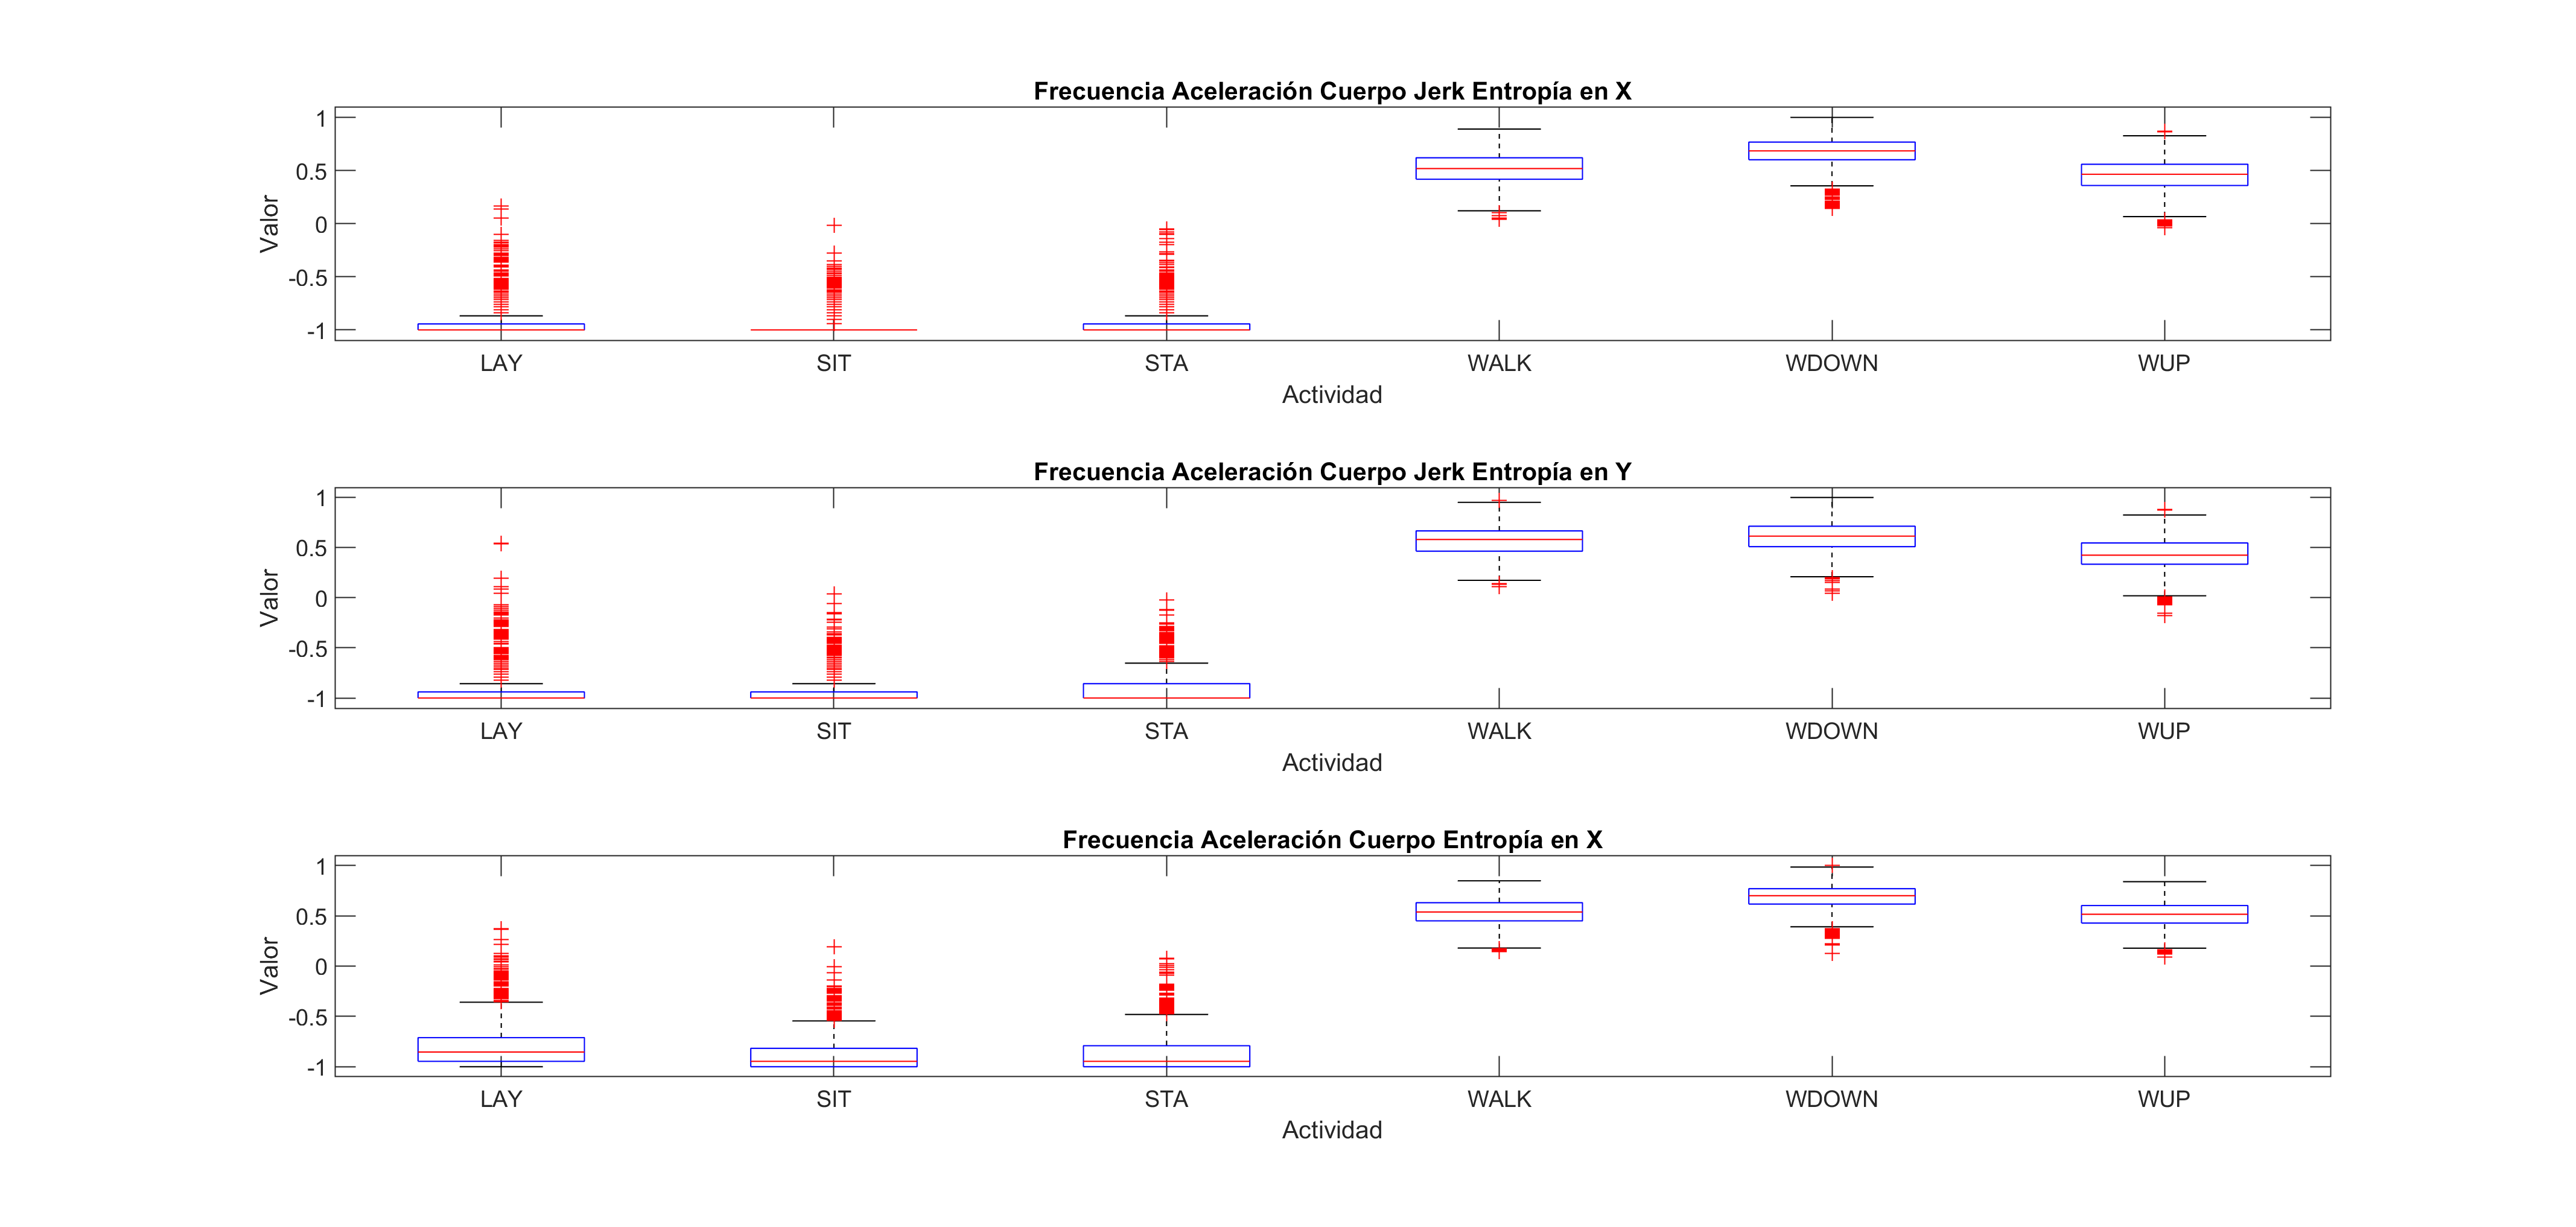
\includegraphics[width=1\textwidth]{varianza_frecuencia}
   \caption{Boxplot Características en Frecuencia}
\end{figure}

\begin{figure}[H]
  \centering
    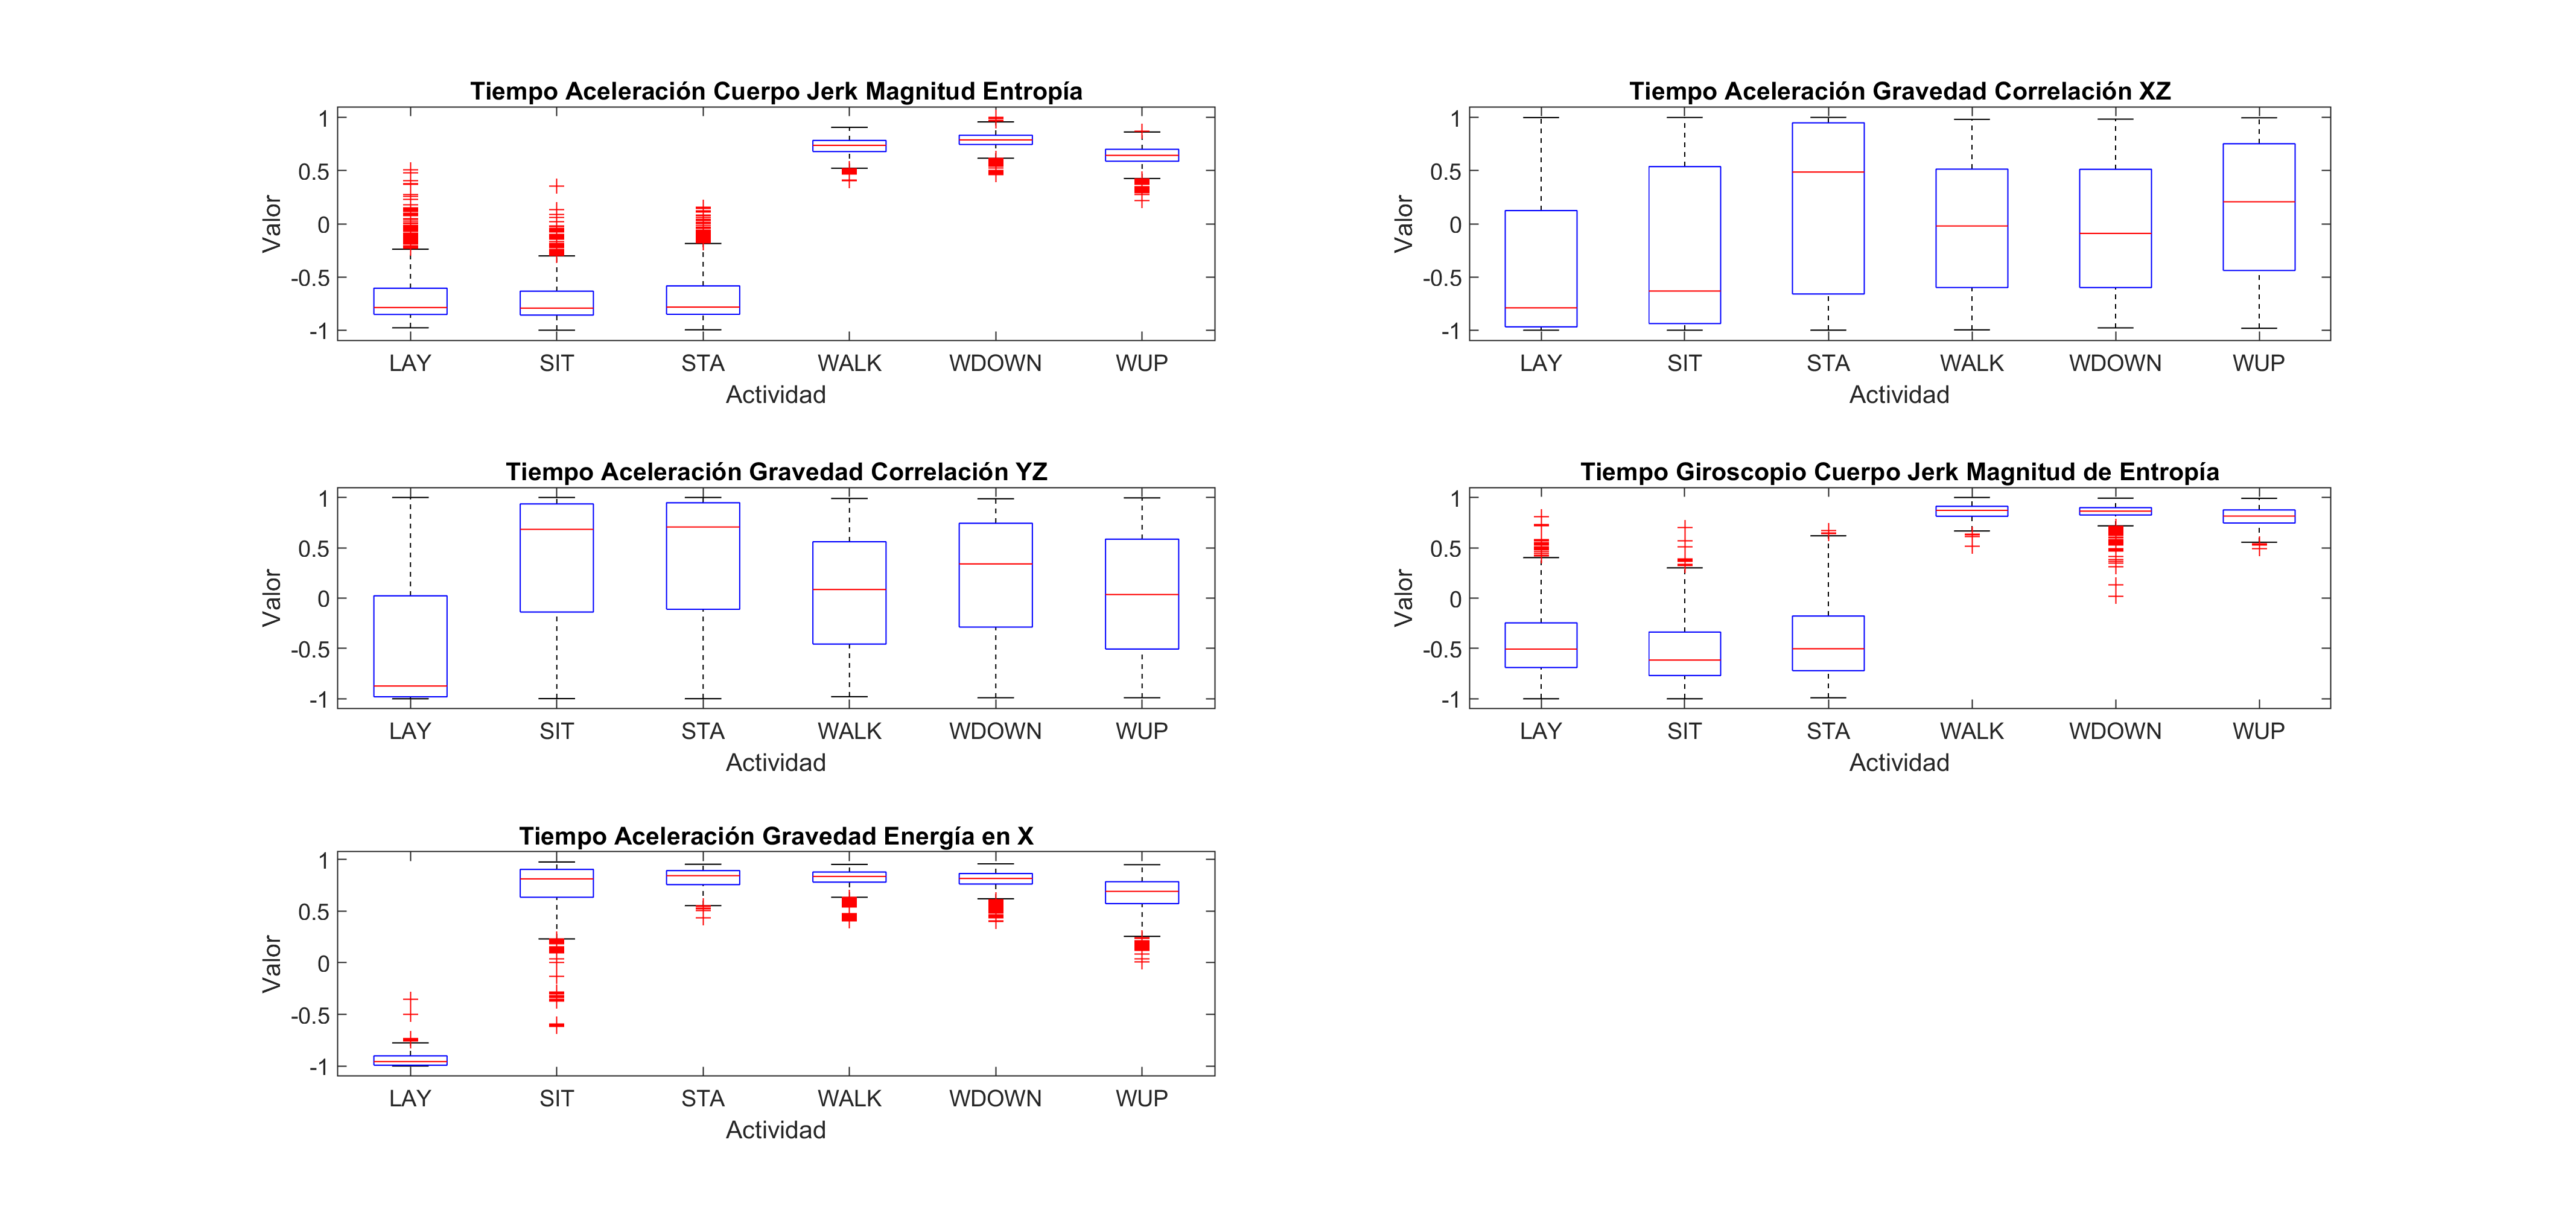
\includegraphics[width=1\textwidth]{varianza_tiempo}
   \caption{Boxplot Características en Tiempo}
\end{figure}

\par
\medskip
\noindent


\section{Elección del Clasificador}

En cuanto a cuál es el mejor clasificador (incluyendo el kernel) más apropiado para la clasificación de actividad humana usando acelerometros de smartphones se deben tener en cuenta dos cosas, la exactitud a la hora de clasificar y, además, el tiempo de computación del clasificador, como se puede observar en la tabla.

Para la clasificación se utilizaron las primeras 50 componentes principales. Los resultados se pueden observar en las siguientes tablas.

\begin{figure}[H]
  \centering
    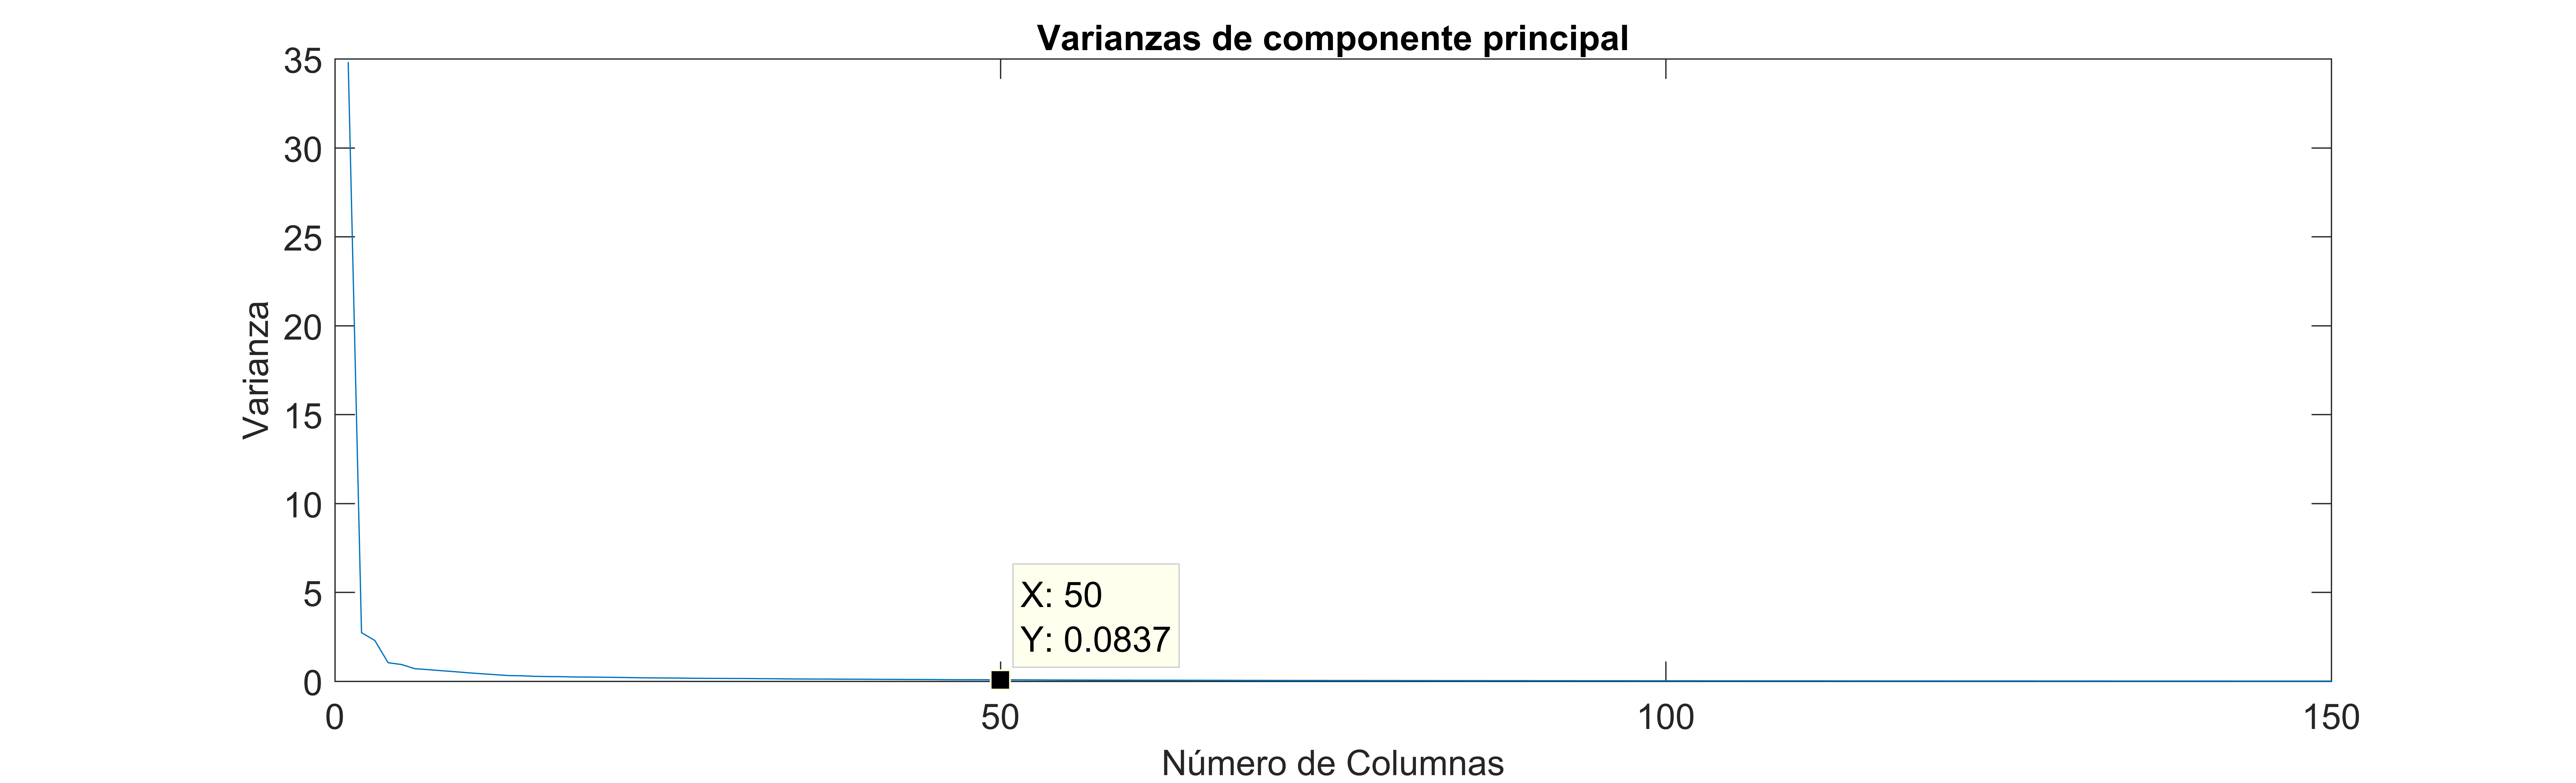
\includegraphics[width=1\textwidth]{pca}
   \caption{Varianzas de las componentes principales}
\end{figure}

\begin{table}[H]
  \begin{tabular}{|l|l|l|l|l|l|l|}
    \hline
    \multirow{2}{*}{Clasificador} &
      \multicolumn{3}{c}{PCA} &
	\multicolumn{3}{|c|}{NO PCA} \\
    & t train  & \% train & \% testing & t train  & \% train & \% testing \\
    \hline
    Cubic SVM & 18 s & 97.6\% & 91.8\% & 127.3 s & 99.1\% & 97.8\% \\
    \hline
    Linear SVM & 16.2 s & 95.3\% & 90.3\% & 61.1 s & 98.3\% & 95.1\% \\
    \hline
    M.G. SVM & 21.8 s & 97.3\% & 94.1\% & 221.3 s & 97.9\% & 91.2\% \\
    \hline
Quadratic SVM & 15.9 s & 97.4\% & 94.2\% & 68.3 s & 98.9\% & 96.7\% \\
    \hline
    Complex DT & 14 s & 86.5\% & 83.5\% & 52.2 s & 93.9\% & 90\% \\
    \hline
    Simple DT & 9.9 s & 63.3\% & 64.3\% & 62.5 s & 78.5\% & 71\% \\
    \hline
Medium DT & 8.1 s & 82.3\% & 80\% & 42.3 s & 91.3\% & 89.4\% \\
    \hline
    Weighted KNN & 10.6 s & 95.2\% & 94\% & 338.2 s & 96.3\% & 91.1\% \\
    \hline
    Fine KNN & 10.5 s & 94.6\% & 87\% & 115.1 s & 96.7\% & 92.3\% \\
    \hline
Cosine KNN & 10 s & 95.3\% & 90\% & 227 s & 96.1\% & 89.4\% \\
    \hline
  \end{tabular}
\label{Efectos de PCA}
\caption{Efectos de PCA}
\end{table}

Si el sistema debe cumplir con una exactitud mayor al 90\%, se prioriza el clasificador que haya requerido menos recursos para lograr a esta exactitud en la clasificación, por lo tanto se puede decir que el clasificador más apropiado (implementando PCA) es el SVM con kernel cúbico; y el mejor clasificador sin implementar PCA fue el árbol de decisiones con el kernel Medium (en cuanto a costo computacional).


\section{Posicion del Sensor}

\begin{table}[H]
  \begin{tabular}{|l|l|l|l|l|l|l|}
    \hline
    \multirow{2}{*}{Clasificador} &
      \multicolumn{2}{c}{Kaggle} &
	\multicolumn{2}{c}{Sensor Cintura} &
	\multicolumn{2}{|c|}{Sensor Muñeca} \\
    & \% train  &  \% testing & \% train & \% testing  & \% train & \% testing \\
    \hline
    Cubic SVM & \cellcolor{blue!25}97.6\% & 91.8\% & \cellcolor{blue!25}92.7\% & \cellcolor{blue!25}89 \% & \cellcolor{blue!25}78.3\% & 72.1\% \\
    \hline
    Linear SVM & 95.3\% & 90.3\% & 86.9\% & 81.8\% & 67.3\% & 61.6\% \\
    \hline
    M.G. SVM & 97.3\% & 94.1\% & 88\% & 85 & 72\% & 65.5\% \\
    \hline
Quadratic SVM & 97.4\% & \cellcolor{blue!25}94.2\% & 91.7\% & 87.1 \% & 76\% & 62.1\% \\
    \hline
    Complex DT & 86.5\% & 83.5\% & 82.9\% & 78.4 \% & 52\% & 51.6\% \\
    \hline
    Simple DT & 63.3\% & 64.3\% & 72.3\% & 62.5 \% & 66.1\% & 65.5\% \\
    \hline
Medium DT &  82.3\% & 80\% & 82.4\% & 79.4 \% & 60.9\% & 52.1\% \\
    \hline
    Weighted KNN & 95.2\% & 94\% & 81.1\% & 76.3\% & 74.3\% & 71.6\% \\
    \hline
    Fine KNN & 94.6\% & 87\% & 82.3\% & 81\% & 78.2\% & \cellcolor{blue!25} 75.5\% \\
    \hline
Cosine KNN & 95.3\% & 90\% & 76.9\% & 70\% & 69.6\% & 65.5\% \\
    \hline
  \end{tabular}
\caption{Comparación entre locaciones del sensor}
\end{table}

\par
\medskip
\noindent
En cuanto a la posición del sensor se observa claramente que la mejor posición para poner el sensor para clasificación de actividad humana entre la cintura y la muñeca, es la cintura, ya que la exactitud en la validación de los clasificadores es bastante mayor que en la de la muñeca.


Teniendo en cuenta que el alcance futuro del proyecto es aportar a la investigación de monitoreo remoto de pacientes con enfermedades motoras, este proceso debe hacerse en tiempo real (con el hardware de un smartphone), esto quiere decir que el proceso de segmentación y extracción de características debe requerir un bajo costo computacional para que esto sea posible. Además, reducir el número de características ayuda también a que el clasificador se entrene y clasifique en un tiempo mucho menor. El costo computacional fue medido con el número de procesos para llevar a cabo la clasificación para cada clasificador:

\begin{table}[H]
\begin{center}
  \begin{tabular}{|l|l|l|l|l|l|l|}
    \hline
 \textbf{Clasificador} & 
 \multicolumn{2}{c}{561 Características} &
	\multicolumn{2}{|c|}{280 Características} \\
    \hline
	& t (s) & vel (proc/sec)& t (s) & vel (proc/sec) \\
\hline
    Linear SVM & 43.3 & 3800 & 5.84 & 6000 \\
    \hline
    Quadratic SVM & 51.6 & 2100 & 6.2 & 3800 \\
    \hline
    Cubic SVM & 102 & 1400 & 9.5 & 5400\\
    \hline
     MG SVM & 188.4 & 760 & 13.8 & 4100 \\
    \hline
    Simple DT & 47.3 & 28000 & 7.46 & 28000\\
    \hline
    Medium DT & 29.8 & 22000 & 5.7 & 11000\\
    \hline
    Complex DT & 38 & 22000 & 7.25 & 9100\\
    \hline
     Fine KNN & 108 & 230 & 4 & 2200 \\
    \hline
    Cosine KNN & 219 & 220 & 7.8 & 2200 \\
    \hline
    Weighted & 321 & 250 & 9.8 & 2400 \\
    \hline
  \end{tabular}
\label{Efectos de PCA}
\caption{Diferencias de tiempos entre Número de características}
\end{center}
\end{table}

Como se puede observar al reducir el número de características a la mitad, disminuye el tiempo de entrenamiento de los clasificadores sustancialmente, de hecho en algunos casos el tiempo es disminuido más de 20 veces.

Para observar y comparar los resultados con respecto a los trabajos realizados anteriormente, se realizó la siguiente tabla en comparación con el mejor resultado obtenido en la competencia realizada por Kaggle:

\begin{table}[H]
\begin{center}
  \begin{tabular}{|l|l|l|l|l|l|l|}
    \hline
 \textbf{} & \textbf{Plataforma Kaggle} & \textbf{Extracción Kaggle}& \textbf{Protocolo Experimental}\\
    \hline
    Exactitud & 99.3\% & 99.1\% & 92.7\% \\
    \hline
  \end{tabular}
\label{Comparacion}
\caption{Exactitudes entre los resultados de Kaggle, el sistema para la extracción de Kaggle y el sistema para el protocolo experimental}
\end{center}
\end{table}

Como se puede observar en la tabla 6.4 los resultados obtenidos para el sistema de clasificación implementado fueron similares a los mejores resultados de la competencia.

\chapter{CONCLUSIONES Y RECOMENDACIONES}

\begin{itemize}
\item Se implementó un sistema de clasificación para varios clasificadores y se obtuvo como mejor clasificador SVM con kernel cúbico para las 3 implementaciones, base datos Kaggle, Protocolo experimental cintura, protocolo experimental muñeca, con una exactitud de 97.6\%, 97.7\% y 78.3\% respectivamente.
\item Se diseñó un protocolo experimental con dos posiciones diferentes del sensor en el cuerpo (muñeca y cintura), obteniendo mejores resultados para el sensor localizado en la cintura con una exactitud promedio de los clasificadores de 77\%. Estos resultados se deben a que el movimiento de las articulaciones (en este caso el brazo) es más dependiente de la persona que realice las actividades, por lo tanto hace que esta locación del sensor sea más independiente del modelo encontrado por el clasificador.
\item Se comprobó que el tiempo de entrenamiento de los clasificadores se puede disminuir sustancialmente reduciendo el número de características sin tener mayores pérdidas en la exactitud del clasificador para en posteriores trabajos realizar la clasificación en tiempo real.
\item Se compararon los resultados de la implementación del sistema con los mejores resultados de la competencia realizada por Kaggle obteniendo resultados muy similares en cuanto a la exactitud del clasificador. 
\item Como una recomendación para posteriores estudios en pacientes con Parkinson, se deben tener en cuenta distintos factores a la hora de seleccionar un transductor para el análisis de temblores. Hay que considerar las características cinemáticas del temblor para que el transductor tenga la suficiente sensibilidad, rango de amplitud y rango de frecuencia para registrar el temblor con buena facilidad. El transductor también debe ser lo suficientemente pequeño y liviano par montarse de manera segura en la parte del cuerpo deseada, sin impedir la tarea a realizarse.La mayoría de los temblores que se presentan en las distintas partes del cuerpo tienen un ancho de banda <10 Hz.\cite{elble2016using}
\end{itemize}


\bibliography{biblio} 
\bibliographystyle{ieeetr}

\chapter{ANEXOS}

\noindent
\textbf{Javier Ricardo Becerra Bedoya}

\noindent
\textbf{Pontificia Universidad Javeriana, Bogotá}

\noindent
\textbf{Trabajo de grado: Clasificación de actividad humana con acelerómetros de Smartphones.}

Bogotá,   \indent   \indent de  Septiembre del 2017

\medskip
\noindent
\textbf{Introducción y propósito}

Yo, Javier Ricardo Becerra Bedoya, estudiante de ingeniería electrónica de la Pontificia Universidad Javeriana de Bogotá, en la realización del trabajo final del pregrado, he solicitado su colaboración y participación voluntaria, en la recolección de datos de movimiento mediante un Smartphone ubicado en dos lugares distintos del cuerpo (cintura y brazo). Lo anterior, con el objetivo de realizar un sistema  de clasificación de actividad humana automático, que aportará a la investigación en el monitoreo de enfermedades que afectan la capacidad motora, como el Párkinson, para buscar una mejora en la calidad de vida de estos pacientes.
\par
\medskip
\noindent
Mediante este documento, yo, garantizo que no será vulnerada su integridad física ni mental y que sus datos serán tratados confidencialmente, teniendo en cuenta que este estudio se cataloga como investigación de riesgo mínimo según la RESOLUCIÓN No 008430 DE 1993 del Ministerio de Salud de Colombia. 

\par
\medskip
\noindent
\textbf{Procedimiento a realizar} 

\par
\medskip
\noindent
Se le entregará al voluntario un Smartphone Samsung Galaxy SII con dos accesorios para localizarlo en dos partes distintas del cuerpo (una riñonera y banda para el brazo). Una vez haya sido localizado en una de las dos partes del cuerpo se procederá a realizar el protocolo de pruebas indicado en la tabla con los tiempos designados, grabando en tiempo real los datos recolectados por el acelerómetro y giroscopio del celular.  Se le indicará al voluntario el recorrido exacto para cada actividad y los tiempos en los que debe ir cambiando de la una a la otra. El procedimiento debe ser repetido para la otra posición del Smartphone.


\begin{table}[h!]
\begin{center}
\begin{tabular}{ |c|c|c|c|c|c| } 
\hline
\textbf{No.} & \textbf{Estáticas} & \textbf{Tiempo (S)} & \textbf{No.} & \textbf{Dinámicas} & \textbf{Tiempo (S)} \\
\hline
0 & Comienzo (de pie) & 0 & 7 & Caminar (1) & 15 \\ 
1&  Reposo (De pie) & 15 & 8 & Caminar(2) & 15\\ 
2&  Sentar & 15 & 9 & Bajar Escaleras (1) & 36\\ 
3&  De Pie & 15 & 10 & Subir Escaleras (2) & 36\\ 
4&  Acostarse & 15 & 11 &  & \\ 
5&  Sentar & 15 & 12 &  & \\ 
6&  Acostarse & 15 & 13 &  & \\ 
\hline
\hline
&   &  &  & \textbf{Total} & \textbf{192}\\ 
\hline
\end{tabular}
\caption{Protocolo de actividades a realizar}
\end{center}
\end{table}

\par
\medskip
\noindent
\textbf{Consentimiento informado}

\par
\medskip
\noindent
Yo,  \indent   \indent  \indent   \indent \indent   \indent  \indent   \indent  \indent   \indent  \indent   \indent he leído y escuchado los propósitos, objetivos y procedimientos a realizar en el presente estudio, he tenido la oportunidad de preguntar sobre este y me ha sido brindada una respuesta óptima. Decido participar voluntariamente en la toma de los datos necesarios y tengo claridad de que mis datos serán tratados de manera confidencial y con fines académicos. Además, soy consciente de que me puedo retirar del estudio en el momento que lo desee y que el procedimiento planteado no afecta mi integridad física ni mental. 

\par
\medskip
\medskip
\medskip
\noindent
\textbf{Firma: }

\par
\medskip
\noindent
\textbf{Fecha: } 

\par
\medskip
\noindent
\textbf{Documento de identidad: } 

\end{document}